\documentclass[twoside, openright, titlepage, fleqn, headinclude, 11pt, a4paper, BCOR5mm, footinclude]{book}

%-----------------------------------------------------------------

\usepackage[utf8]{inputenc}
\usepackage[T1]{fontenc}
\usepackage[italian]{babel}
\usepackage[pdftex]{graphicx}
\usepackage[square, numbers]{natbib}
\usepackage[Lenny]{fncychap}
\usepackage[nottoc, notlof]{tocbibind}
\usepackage[unicode]{hyperref}
\usepackage[fixlanguage]{babelbib}
\usepackage{amsfonts, amsmath, geometry, xcolor, url, caption, perpage, datetime, placeins}

%-----------------------------------------------------------------

\newcommand{\HRule}{\rule{\linewidth}{0.5mm}}

\newdateformat{monthyear}{\monthname[\THEMONTH] \THEYEAR}

\captionsetup{format=hang,font=small}

\MakePerPage{footnote}

\graphicspath{{img/}}

\selectbiblanguage{italian}

%-----------------------------------------------------------------

\hypersetup{
	colorlinks,
	citecolor=black,
	filecolor=black,
	linkcolor=black,
	urlcolor=blue
}

%-----------------------------------------------------------------

\begin{document}

	\frenchspacing
	\raggedbottom
	\pagenumbering{roman}
	\pagestyle{plain}
	
	\begin{titlepage}
\vspace{2cm}
	\begin{center}
		{\Large {UNIVERSIT\`{A} DEGLI STUDI DI FIRENZE}}
	\end{center}
	
	\begin{center}
		{\normalsize {Facoltà di Scienze Matematiche, Fisiche e Naturali}}
	\end{center}

	\begin{center}
		{\normalsize Corso di Laurea Magistrale in Informatica}
	\end{center}
\vspace{1cm}
	\begin{center}
		
\includegraphics[scale=1]{unifi.jpg}
	\end{center}
\vspace{2cm}
	\begin{Huge}
		\begin{center}
			Progetto per il corso di\\ ANALISI QUANTITATIVA DEI SISTEMI
		\end{center}
	\end{Huge}
\vspace{1cm}
	\begin{center}
	\Large \textbf{GRUPPO 3}
	\end{center}
	\begin{center}
		{\large Bernini Riccardo matr. 5435313}
	\end{center}
    \begin{center}
		{\large Papini Tommaso matr. 5537529}
	\end{center}
\vspace{1.2cm}
	\begin{center}
		A.A. 2012/2013
	\end{center}
\end{titlepage}
	
	\tableofcontents %\addtocontents{toc}{~\hfill\textbf{Pagina}\par}
	\listoffigures
	
	\cleardoublepage
	\pagenumbering{arabic}
	\pagestyle{headings}
	
	\chapter{Introduzione} \label{chap:introduzione}
	
	\mylettrine{C}{hiunque} abbia la seppur minima passione per la musica avrà sicuramente sentito parlare, al giorno d'oggi, del formato (o più in generale, della tecnologia) \textit{MP3}. Sicuramente i più sapranno che l'MP3 è un formato audio digitale che permette di memorizzare file audio, come canzoni, utilizzando molto meno spazio rispetto ai precedenti formati, pur mantenendo una buona qualità sonora: molti ricorderanno l'avvento dei primi lettori CD MP3, che permettevano di registrare e riprodurre centinaia di canzoni in un unico CD da 700 MB, al contrario delle massimo 20 canzoni che si potevano masterizzare in qualità CD (di queste differenze di formati e qualità audio parleremo ampiamente più avanti).\\
	La parola MP3 è spesso associata ai concetti di ``Internet'', ``frode'' o ``pirateria informatica'', dal momento che la sua venuta ha dato il via, o comunque incentivato, il download di enormi quantità di dati audio, spesso senza possedere alcuna licenza ed in modo certamente illegale.\\
	\\
	Ma a parte questi aspetti di conoscenza comune, pochi sanno veramente cos'è l'MP3 e come funzioni ed ancor meno sono quelli che si prendono la briga di spiegarlo. Con questo elaborato ci prefiggiamo quindi l'obiettivo di descrivere come e perché è nato l'MP3 e come esso funzioni, senza perdersi troppo nei dettagli tecnici ma fornendo comunque un'idea generale della tecnologia MP3.
	
	\section{Definizioni} \label{sec:definizioni}
		Senza dilungarci troppo nei dettagli, diamo alcune definizioni iniziali che faciliteranno la comprensione di questa relazione.
		
		\begin{defi} \label{defi:mp3}
			L'\emph{\textbf{MP3}} (ovvero \emph{\textbf{M}oving \textbf{P}icture} Expert Group-1/2 Layer \textbf{III}), detto anche \emph{MPEG-1/2 Layer III}, è un algoritmo di compressione audio di tipo \emph{lossy}, sviluppato dal gruppo \emph{MPEG}.
		\end{defi}
		
		Avendo introdotto, nella definizione precedente, il concetto di algoritmo \textit{lossy}, definiamo adesso cos'è un algoritmo di compressione \textit{lossy} e cos'è invece uno \textit{loosless}:
		
		\begin{defi} \label{defi:lossy}
			Un algoritmo di compressione \emph{\textbf{lossy}} è un metodo di codifica che comprime i dati scartandone alcuni. Tramite il processo di decodifica, quindi, non sarà possibile riottenere i dati originali.
		\end{defi}
		
		\begin{defi} \label{defi:loosless}
			Un algoritmo di compressione \emph{\textbf{loosless}} è un metodo di codifica che comprime i dati senza perderne alcuno. Tramite opportuna decodifica sarà quindi possibile ottenere nuovamente i dati originali.
		\end{defi}
		
		Già da queste definizioni possiamo dedurre che l'MP3 è un algoritmo di compressione audio che, comprimendo i dati, scarta alcune informazioni, al fine di rendere il file finale molto più leggero e maneggevole.
		
	\section{Cenni di compressione di dati} \label{sec:cenni_compressione_dati}
		
		Nel 1949 Claude E. Shannon provò, all'interno del suo articolo ``A Mathematical Theory of Communication'', che esiste un limite teorico alla compressione dei dati senza perdere informazione, ovvero comprimendo i dati con algoritmi loosless. Questo limite, detto \textit{tasso d'entropia}, dipende dalla probabilità di trovare determinate sequenze di bit: è possibile comprimere i dati con un tasso di compressione vicino al tasso d'entropia ed è matematicamente impossibile fare meglio.\\
		Per ottenere una maggior compressione dei dati è necessario utilizzare algoritmi lossy e quindi accettare di perdere parte dei dati.\\
		\\
		Di seguito esporremo tre codifiche di tipo loosless molto semplici, una delle quali, come vedremo, utilizzata anche all'interno dell'algoritmo di compressione e decompressione MP3.
		
		\subsection{Run-Length Encoding} \label{subsec:run-length_encoding}
		
			L'algoritmo di compressione loosless \textit{Run-Length Encoding} (o semplicemente \textit{RLE}) consiste nel codificare le varie sequenze di bit consecutivi aventi lo stesso valore come coppie, dove il primo elemento rappresenta il valore di quei bit e il secondo elemento indica il numero di bit che compongono la sequenza, ovvero la lunghezza della sequenza. In Figura \ref{fig:run-length_encoding} possiamo vedere un esempio della codifica RLE. Questa codifica è ideale per dati con lunghe sequenze di bit identici (quindi sconsigliato per dati casuali).
			
			\begin{figure}[h!]
				\centering
					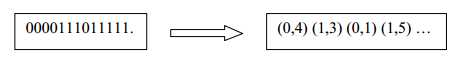
\includegraphics[scale=1]{run-length_encoding.png}
				\caption{Algoritmo di compressione Run-Length Encoding.}
				\label{fig:run-length_encoding}
			\end{figure}
			
		\subsection{Move-To-Front} \label{subsec:move-to-front}
			
			La codifica \textit{Move-To-Front} (o \textit{MTF}) si basa sul concetto di entropia ed infatti è ottimizzata quando la lettura di un carattere aumenta le probabilità di trovare lo stesso carattere subito dopo.\\
			L'algoritmo inizia codificando le lettere dell'alfabeto secondo l'ordine usuale (da 0 a 25). Quindi ogni carattere che viene incontrato viene spostato in cima alla lista. In generale, elementi in cima alla lista vengono codificati con meno bit, mentre quelli verso il fondo richiedono più bit.\\
			\\
			Se ad esempio prendiamo la parola ``BANANAAA'', la codifica MTF di questa parola sarà quella in Tabella \ref{tab:move-to-front}.
			
			\begin{table}[h!]
				\centering
				\begin{tabular}{|l|l|c|}
					\multicolumn{1}{c}{\textbf{Sequenza}} & \multicolumn{1}{c}{\textbf{Codifica}} & \multicolumn{1}{c}{\textbf{Lista}}\\
					\hline
					b & 1 & abcdefghijklmnopqrstuvwxyz\\
					\hline
					ba & 1, 1 & bacdefghijklmnopqrstuvwxyz\\
					\hline
					ban & 1, 1, 13 & abcdefghijklmnopqrstuvwxyz\\
					\hline
					bana & 1, 1, 13, 1 & nabcdefghijklmopqrstuvwxyz\\
					\hline
					banan & 1, 1, 13, 1, 1 & anbcdefghijklmopqrstuvwxyz\\
					\hline
					banana & 1, 1, 13, 1, 1, 1 & nabcdefghijklmopqrstuvwxyz\\
					\hline
					bananaa & 1, 1, 13, 1, 1, 1, 0 & anbcdefghijklmopqrstuvwxyz\\
					\hline
					bananaaa & 1, 1, 13, 1, 1, 1, 0, 0 & anbcdefghijklmopqrstuvwxyz\\
					\hline
				\end{tabular}
				\caption{Algoritmo di compressione Move-To-Front.}
				\label{tab:move-to-front}
			\end{table}
		
		\subsection{Codifica di Huffman} \label{subsec:codifica_huffman}
			
			Il concetto di entropia viene ampiamente applicato anche alla codifica di Huffman che, come vedremo più avanti, viene utilizzata all'interno dell'algoritmo di compressione MP3. L'idea che sta alla base della codifica di Huffman è quella di codificare con meno bit i caratteri più frequenti. La probabilità di incontrare determinati caratteri dev'essere determinata a priori (ad esempio analizzando i dati che si vogliono comprimere). Successivamente, in base alle probabilità calcolate, si assegnano codifiche più corte ai caratteri più frequenti e si memorizzano le associazioni carattere-codifica in una tabella, detta \textit{tabella di Huffman}, necessaria per la successiva decodifica dei dati. Come possiamo vedere in Figura \ref{fig:huffman}, la tabella di Huffman può essere rappresentata anche come un albero binario.
			
			\begin{figure}[h!]
				\centering
					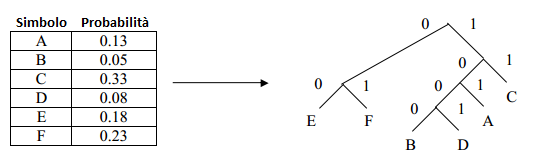
\includegraphics[scale=1]{huffman.png}
				\caption{Codifica di Huffman.}
				\label{fig:huffman}
			\end{figure}
		
	\chapter{Modellazione concettuale} \label{chap:modellazione_concettuale}
	
	A partire dalla pseudo-narrazione derivante dalla descrizione, dagli obiettivi di questo progetto e dall'analisi dei \textit{dataset} utilizzati si può ottenere uno schema concettuale che, attraverso una serie di entità e le relazioni tra esse, possa modellare dettagliatamente la realtà che ci proponiamo di analizzare.\\
	Gli obiettivi da tener presente nella costruzione dello schema concettuale sono: da una parte la necessità di soddisfare i requisiti utente; dall'altra la necessità di consistenza dello schema concettuale con gli schemi delle sorgenti operazionali.\\
	L'approccio metodologico alla progettazione concettuale utilizzato è l'approccio guidato dai dati: lo schema concettuale viene cioè definito in funzione della struttura delle sorgenti stesse, evitando così il complesso compito di stabilire il legame con esse a posteriori.
	
	\begin{figure}[h!]
		\centering
			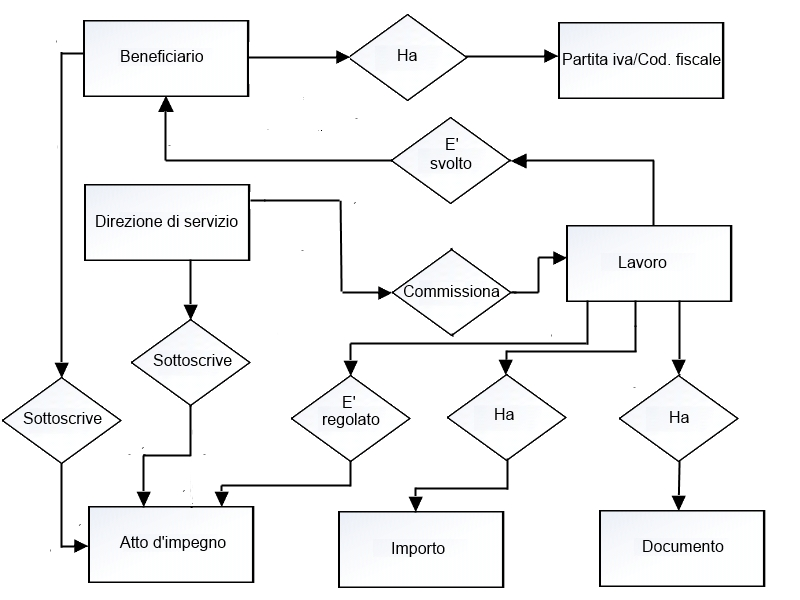
\includegraphics[scale=0.5]{schemaconcettuale.jpg}
		\caption{Schema-concettuale.}
		\label{fig:schemaconcettuale}
	\end{figure}
	
	Una modellazione di questo tipo fornisce inoltre le basi per la costruzione di un'ontologia e una conseguente interrogazione dei dati da un punto di vista semantico.\\
	Il passaggio successivo consiste nell'attribuzione di un \textbf{URI} (\textit{Uniform Resource Identifier}) alle entità coinvolte nello schema, in modo tale da creare una correlazione tra i riferimenti del modello e la posizione reale dei dati.\\
	\\
	Lo schema concettuale presentato può essere successivamente tradotto in uno schema entità-relazione più appropriato, che prende il nome di \textit{Dimensional Fact Model}. Questo modello concettuale è specificatamente concepito per fungere da supporto alla progettazione di un \textit{Data Warehouse} e può essere considerato come una specializzazione del modello multidimensionale.\\
	Come si può osservare nella Figura \ref{fig:schemariconciliato}, la rappresentazione generata dal DFM consiste in un insieme di schemi di fatto: gli elementi di base modellati sono i fatti stessi, le misure e le dimensioni.
	
	
	\begin{figure}[h!]
		\centering
			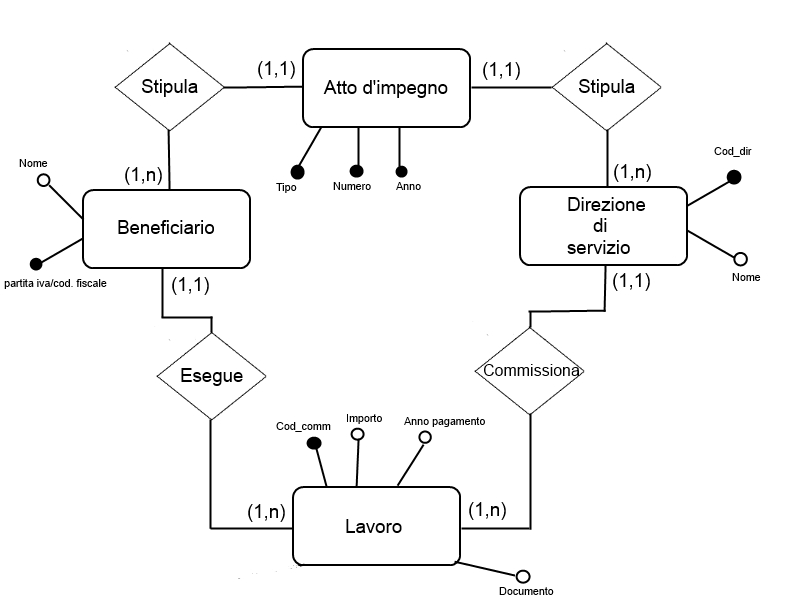
\includegraphics[scale=0.65]{schemariconciliato.jpg}
		\caption{Schema riconciliato.}
		\label{fig:schemariconciliato}
	\end{figure}

	\chapter{Progettazione logica} \label{chap:progettazione_logica}
	
	La progettazione logica permette di determinare lo schema logico del DW. Mentre durante la fase di progettazione concettuale viene ritagliata la porzione del dominio applicativo che dovrà essere considerato, con la fase di progettazione logica si determinano le strutture dati che andranno a rappresentare il DW stesso.\\
	In questo scenario, l'obiettivo primario è quindi di massimizzare la velocità di reperimento dei dati.\\
	
	\section{Schema di fatto} \label{sec:schema_fatto}
		La prima fase della progettazione logica consiste nel dare luogo allo schema che rappresenta l'albero degli attributi. Nello schema seguente (Figura \ref{fig:factschema}) la parte centrale esprime il ``fatto'' (\textit{fact}, in inglese), ovvero ciò a cui è volta la costruzione del modello. I campi del \textit{fatto} rappresentano le misure a cui si fa riferimento per correlare le dimensioni dello schema, che sono ottenute dalla disaggregazione iniziale dei \textit{dataset}.
		
		
		\begin{figure}[h!]
			\centering
				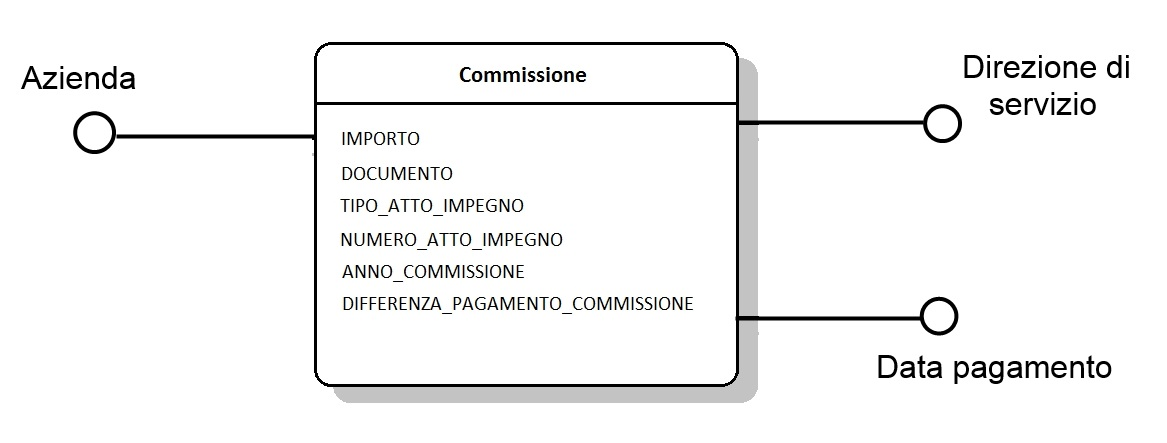
\includegraphics[scale=0.4]{factschema.jpg}
			\caption{Fact-Schema.}
			\label{fig:factschema}
		\end{figure}
		
		
		Uno schema di fatto può essere modellato in ambito relazionale mediante uno schema a stella in cui la cosiddetta \textit{fact table} (\textit{tabella di fatto}) contiene tutte le misure e gli attributi descrittivi direttamente collegati al fatto e nella quale, per ogni gerarchia presente, viene creata una \textit{dimension table} (\textit{tabella dimensionale}) che ne contiene tutti gli attributi.
	
	\section{Schema a stella} \label{sec:schema_stella}
	
		Lo schema a stella rappresenta il rapporto tra le dimensioni del modello e la \textit{fact table} (posta al centro della stella), che andrà a contenere le chiavi inter-dimensionali (indicate nella Figura \ref{fig:starschema} con un simbolo) le quali costituiscono i punti di contatto tra le dimensioni considerate.
		Questo schema a stella permette efficacemente di rappresentare un cubo dimensionale, incentrato sul fatto di interesse del processo decisionale o di analisi. Lo schema ed il cubo rappresentano quindi un insieme di eventi, descritti quantitativamente da misure numeriche. Ogni asse del cubo (ogni dimensione) rappresenta una possibile dimensione di analisi e ciascuna dimensione può essere vista a più livelli di dettaglio, individuati dagli attributi strutturati in gerarchie.
		
		\begin{figure}[h!]
			\centering
				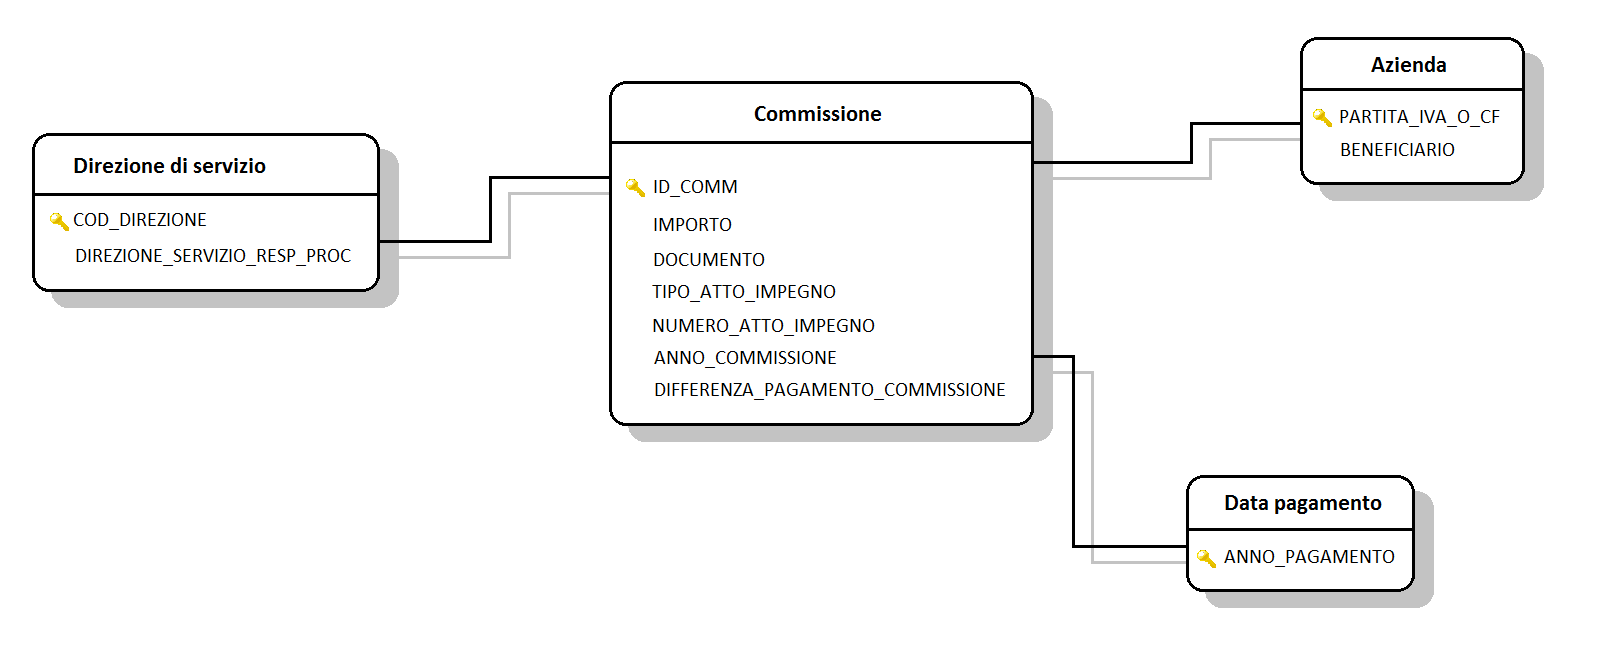
\includegraphics[scale=0.45]{starschema.jpg}
			\caption{Star-Schema.}
			\label{fig:starschema}
		\end{figure}
		
	
	\section{Flat Table} \label{sec:flat_table}
	
		Fin'ora abbiamo parlato di modelli logici a supporto dei nostri dati, come schemi relazionali, concettuali e a stella. Facendo un passo avanti, entriamo quindi nell'ambito dell'implementazione effettiva di questi schemi logici, introducendo il concetto di \textit{Flat Table}: una \textit{Flat Table}, o \textit{Flat-File Database} è un unico file di testo, contenente soltanto dati e delimitatori, che, privo di qualsiasi tipo di riferimento relazionale, rappresenta in concreto il nostro database.\\
		\\
		Nel nostro caso, il file \texttt{.csv} ottenuto come risultato del processo di \textit{Data Integration} sarà allora il supporto ``fisico'' per il nostro database. Questo file, denominato \texttt{Commissioni.csv}, sarà di fatto un unico, enorme file contenente sia i dati della \textit{fact table} sia i dati di tutte le \textit{dimension table} presenti nello schema di fatto. In questo modo viene eliminata ogni tipo di relazione (o se vogliamo, collegamento) tra i dati da analizzare, rendendo necessario più spazio per la memorizzazione ma migliorando notevolmente le tempistiche in fase di analisi.\\
		In Figura \ref{fig:flat_table} possiamo vedere le prime righe e colonne del file \texttt{Commissioni.csv} sopra citato. Per le trasformazioni di \textit{Data Integration} che generano tale file si veda il Capitolo \ref{chap:elaborazione}.
		
		\begin{figure}[h!]
			\centering
				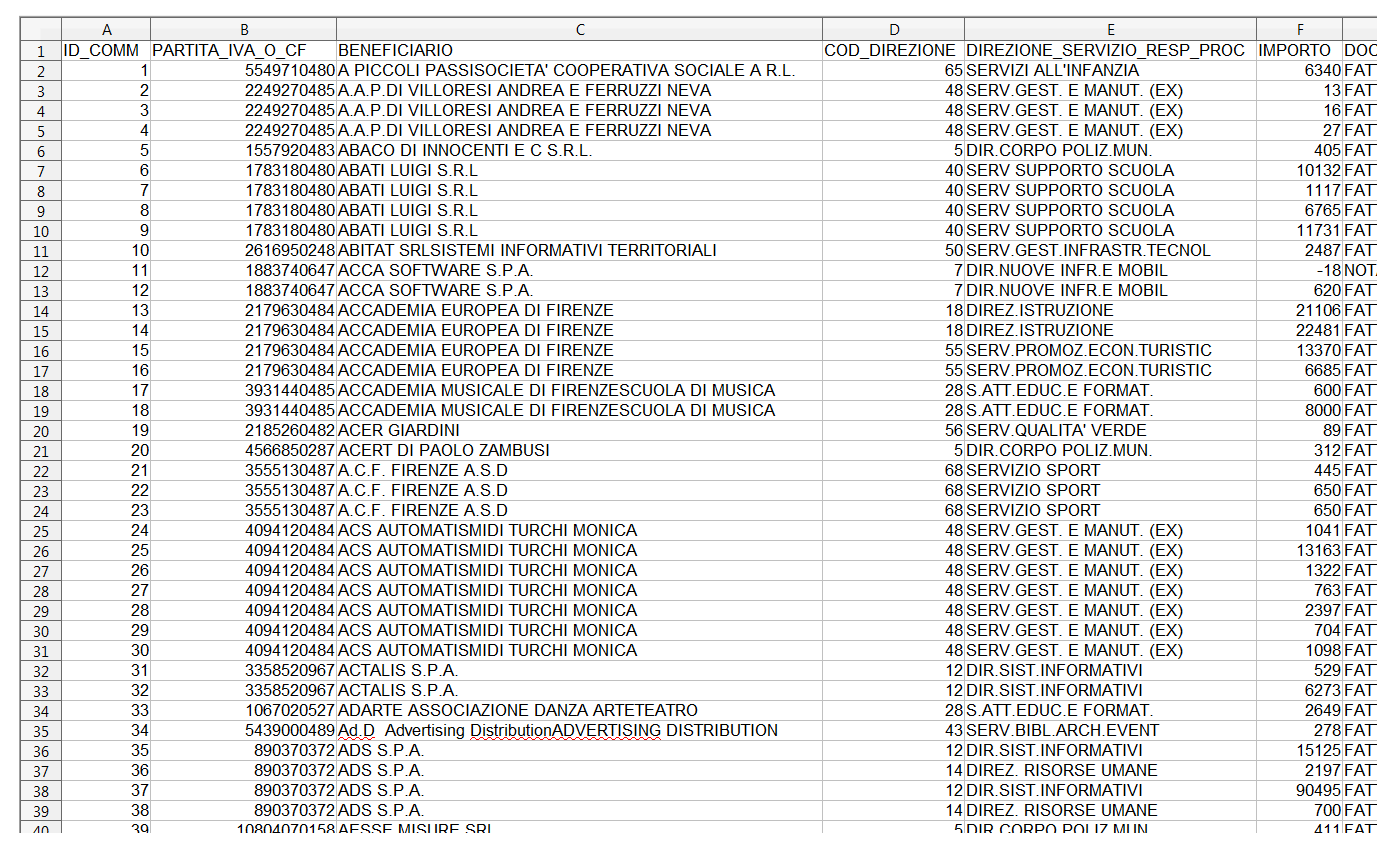
\includegraphics[scale=0.5]{flat_table.png}
			\caption{\textit{Flat Table} finale.}
			\label{fig:flat_table}
		\end{figure}

	\chapter{Elaborazione dei dataset (ETL)} \label{chap:elaborazione}

	Nello sviluppo di questa progetto sono stati usati i \textit{dataset} contenenti il bilancio del 2012 e del 2013 del Comune di Firenze, reperibili sul sito degli \textit{opendata} di Firenze\footnote{\url{http://opendata.comune.fi.it/}}.\\
	Questi \textit{dataset} contengono i dati principali delle fatture dei fornitori del Comune di Firenze per le quali, nel periodo che va dal 26 giugno 2012 (data di entrata in vigore di quanto disposto dall'art.18 del Decreto Sviluppo 2012) fino al 17 dicembre  2012, sono stati sia emessi che quietanzati i mandati di pagamento. Sempre con riferimento a tale articolo, sono stati selezionati gli elementi informativi pubblicati per ciascuna fattura.\\
	\\
	Per quanto riguarda la struttura dei \textit{dataset} essi sono strutturati allo stesso modo, con l'unica eccezione per il bilancio del 2012, che possiede un campo aggiuntivo identificante il numero di mandato (\texttt{NUMERO\_MANDATO}).\\
	Escluso l'eccezione appena introdotta la struttura generale è la seguente:
	\begin{itemize}
		\item \texttt{BENEFICIARIO}: Azienda o privato a cui è stato commissionato un mandato;
		\item \texttt{PARTITA\_IVA\_O\_CF}: partita iva o codice fiscale del beneficiario;
		\item \texttt{IMPORTO}: importo pagato (o ricevuto) dal Comune;
		\item \texttt{ATTO\_DI\_IMPEGNO}: codice contenente il tipo, il numero e l'anno di stipula dell'atto d'impegno;
		\item \texttt{DIREZIONE\_SERVIZIO\_RESP\_PROC}: Direzione di Servizio del Comune di Firenze che ha commissionato il lavoro;
		\item \texttt{DOCUMENTO}: il tipo di documento (fattura/nota di credito).
	\end{itemize}
	
	Lo scopo di questo lavoro è integrare tra loro i \textit{dataset} relativi ai bilanci annuali in modo da poter compiere successivamente delle analisi che non siano ristrette ad un singolo anno, ma che possano confrontare anche i dati su più anni di bilancio. Permetteremo così anche un'analisi temporale dei flussi di pagamento e di credito del Comune di Firenze. Ad esempio cercheremo di integrare i dati in modo tale da permettere il recupero di informazioni come la lista delle aziende a cui sono stati commissionati lavori più lunghi o come variano gli investimenti nei vari settori del Comune di Firenze tra il 2012 ed il 2013.\\
	\\
	Lo strumento utilizzato in questa prima fase è \textit{Kettle}: \textit{Kettle} è un tool di \textit{Data Integration} che permette di specificare, a partire dalle sorgenti dati, una serie di operazioni che produrranno i dati aggregati (o derivati) in output. Sia gli input che gli output possono essere tabelle di Database vere e proprie, oppure, come nel nostro caso, un file \texttt{.csv}, che costituisce un insieme di dati tra loro anche ridondanti.\\
	
	\section{Trasformazione} \label{sec:trasformazione}
		
		Vedremo adesso nel dettaglio la trasformazione \textit{Kettle} che è stata costruita ed utilizzata per questo progetto.
		
		
		\begin{figure}[h!]
			\centering
				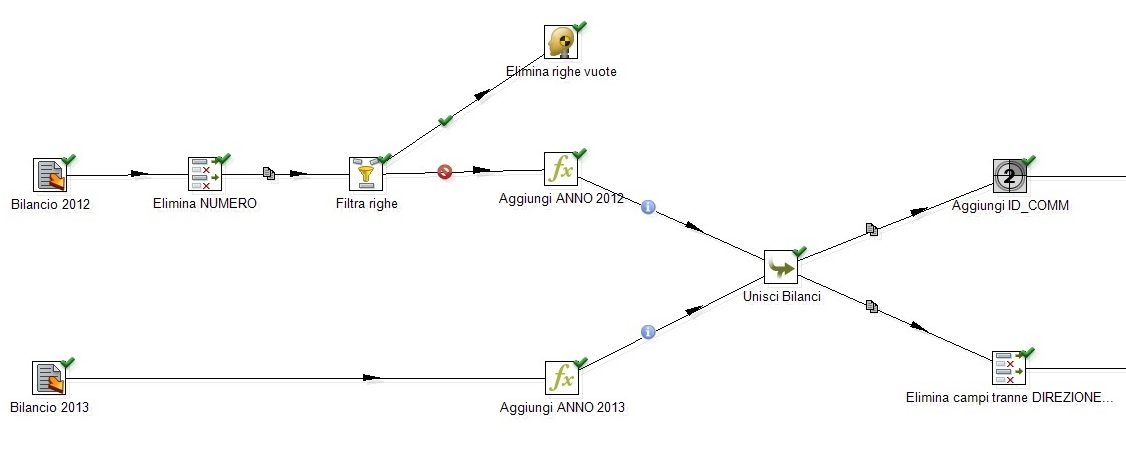
\includegraphics[scale=0.4]{transf1.jpg}
			\caption{Trasformazione Kettle, prima parte.}
			\label{fig:transf1}
		\end{figure}
		
		In questa prima parte della trasformazione (Figura \ref{fig:transf1}) si provvede innanzitutto a caricare le sorgenti dati dell'algoritmo collegate ai file dei vari \textit{dataset} da integrare. Quindi si riportano i due \textit{dataset} ad una struttura comune, eliminando dal bilancio 2012 il campo superfluo \texttt{NUMERO\_MANDATO}, eliminando le eventuali righe vuote ed aggiungendo a ciascun bilancio il relativo anno di appartenenza (campo \texttt{ANNO\_PAGAMENTO}). Infine i due flussi d'input vengono concatenati (funzione di \textit{append}) l'uno di seguito all'altro. Si osservi che in questo caso, come per il resto della trasformazione, l'ordine di concatenazione dei vari flussi è indifferente, in quanto tra gli ultimi step della trasformazione verrà eseguito un ordinamento.\\
		
		\begin{figure}[h!]
			\centering
				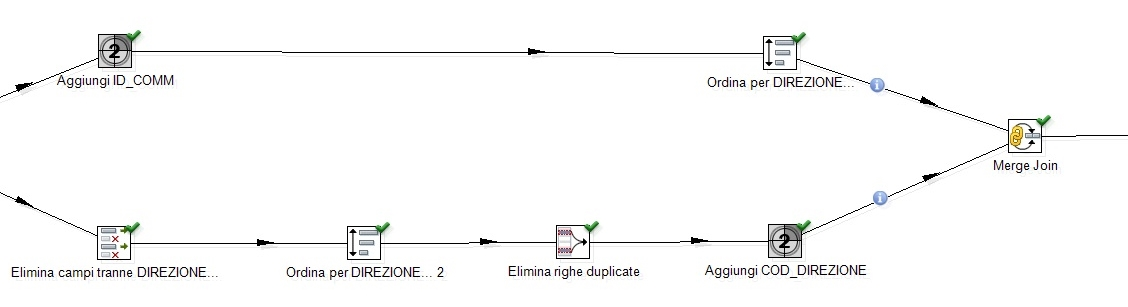
\includegraphics[scale=0.4]{transf2.jpg}
			\caption{Trasformazione Kettle, seconda parte.}
			\label{fig:transf2}
		\end{figure}
		
		A partire dall'unico elenco di commissioni precedentemente generato si generano due flussi di esecuzione (Figura \ref{fig:transf2}): nel primo si provvede ad aggiungere un identificativo per ogni commissione (ovvero per ogni riga presente), chiamato \texttt{ID\_COMM}, e successivamente ad ordinare il tutto rispetto alla direzione di servizio (vincolo necessario per eseguire un merge-join); nel secondo flusso generato, invece, si considerano le sole direzioni di servizio, eliminando ogni altro campo, ed eliminando le voci duplicate (quindi mantenendo una riga per ogni direzione distinta), per poter poi aggiungere un identificativo (\texttt{COD\_DIREZIONE}) ad ognuna di esse. Infine tramite l'utilizzo di un merge-join si provvede ad unire (e non concatenare, come nel caso precedente) i due flussi, così da avere al termine di questi passi per ogni commissione un proprio identificativo e oltre al campo con il nome della direzione di servizio sarà presente anche il codice corrispettivo.\\
		
		\begin{figure}[h!]
			\centering
				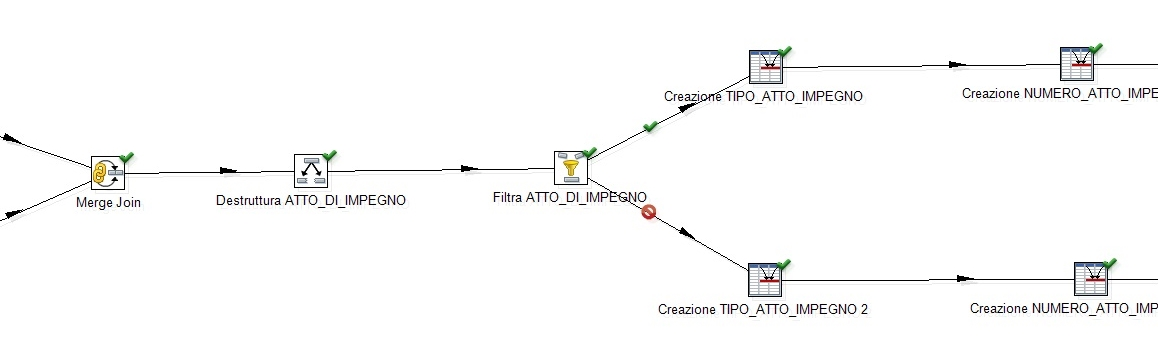
\includegraphics[scale=0.4]{transf3.jpg}
			\caption{Trasformazione Kettle, terza parte.}
			\label{fig:transf3}
		\end{figure}
		
		\begin{figure}[h!]
			\centering
				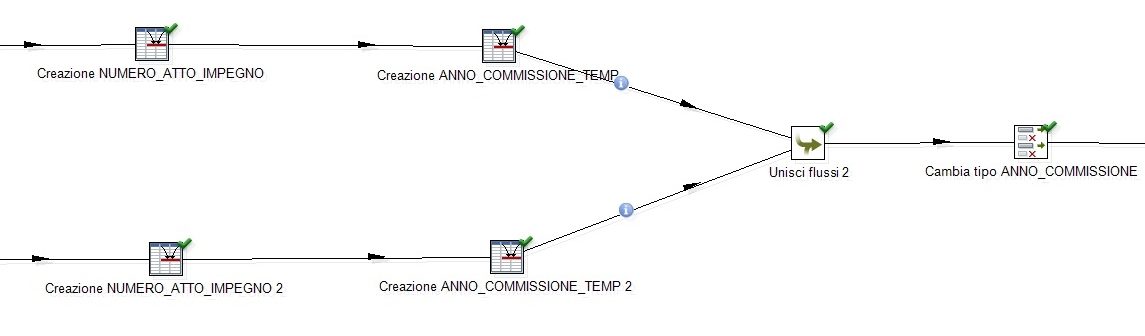
\includegraphics[scale=0.4]{transf4.jpg}
			\caption{Trasformazione Kettle, quarta parte.}
			\label{fig:transf4}
		\end{figure}
		
		I passi presenti nelle Figure \ref{fig:transf3} e \ref{fig:transf4} hanno come obiettivo quello di destrutturare il campo \texttt{ATTO\_DI\_IMPEGNO}, nel quale è tenuto traccia dell'anno di commissione del lavoro, che risulterà utile in fase di analisi. Come si può intuire osservando le figure, l'atto d'impegno è destrutturato nei campi:
		\begin{itemize}
			\item \texttt{TIPO\_ATTO\_IMPEGNO}: suddiviso essenzialmente in \textit{CC} (Consiglio Comunale) e \textit{DD} (Decreto, o Determina, Dirigenziale), indica a che livello è stata deliberata la commissione;
			\item \texttt{NUMERO\_ATTO\_IMPEGNO}: identifica univocamente gli atti d'impegno (si osservi che più commissioni possono riferirsi allo stesso atto d'impegno);
			\item \texttt{ANNO\_DI\_COMMISSIONE\_TEMP}: campo temporaneo in cui vengono registrate le ultime due cifre dell'anno di commissione.
		\end{itemize}
		Al termine di questi passi di destrutturazione vengono riuniti i flussi e viene associato un tipo intero al campo \texttt{ANNO\_DI\_COMMISSIONE\_TEMP}.\\
		
		\begin{figure}[h!]
			\centering
				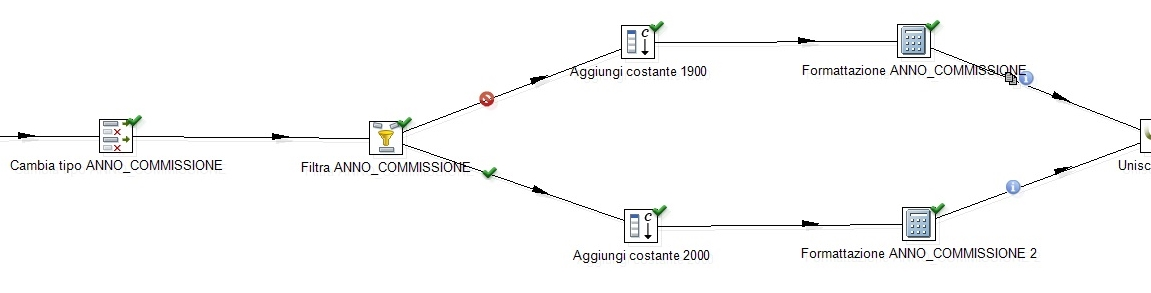
\includegraphics[scale=0.4]{transf5.jpg}
			\caption{Trasformazione Kettle, quinta parte.}
			\label{fig:transf5}
		\end{figure}
		
		I passi rappresentati nella Figura \ref{fig:transf5} hanno invece come obiettivo quello di formattare nel modo corretto l'anno di commissione estratto dall'atto d'impegno: si provvede innanzitutto a discriminare, tramite un filtro, che l'anno sia relativo al 1900 o al 2000 (alcuni atti d'impegno risalgono a più di vent'anni fa!); quindi si generano due flussi di esecuzione, che provvedono ad aggiungere le costanti 1900 o 2000 al campo \texttt{ANNO\_DI\_COMMISSIONE\_TEMP}, generando il nuovo campo \texttt{ANNO\_DI\_COMMISSIONE}; infine si provvede a riunire due flussi.
		
		\begin{figure}[h!]
			\centering
				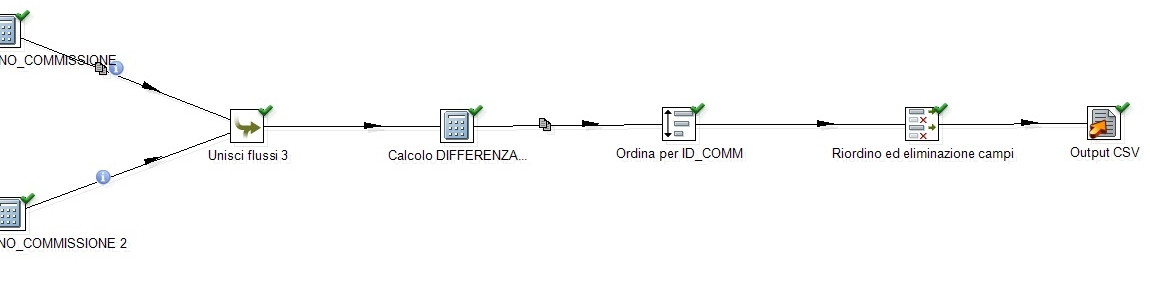
\includegraphics[scale=0.4]{transf6.jpg}
			\caption{Trasformazione Kettle, sesta parte.}
			\label{fig:transf6}
		\end{figure}
		
		Gli ultimi passi della trasformazione (rappresentati in Figura \ref{fig:transf6}) hanno come obiettivo quello di aggiungere un campo derivato, anch'esso necessario in fase d'analisi. Il campo in questione è \texttt{DIFFERENZA\_PAGAMENTO\_COMMISSIONE}, calcolato come differenza tra l'anno di pagamento (associato al bilancio stesso) e l'anno di commissione (precedentemente estratto dall'atto d'impegno).\\
		Le ultime operazioni provvedono ad ordinare tutte le commissioni, ad eliminare i campi non necessari all'analisi e riordinare tra loro quelli utili.\\
		Infine viene generato l'output della trasformazione, \texttt{Commissioni.csv}, che contine tutte le commissioni registrate nei due anni e presenta in quest'ordine i seguenti campi:
		\begin{itemize}
			\item \texttt{ID\_COMM}
			\item \texttt{PARTITA\_IVA\_O\_CF}
			\item \texttt{BENEFICIARIO}
			\item \texttt{COD\_DIREZIONE}
			\item \texttt{DIREZIONE\_SERVIZIO\_RESP\_PROC}
			\item \texttt{IMPORTO}
			\item \texttt{DOCUMENTO}
			\item \texttt{TIPO\_ATTO\_IMPEGNO}
			\item \texttt{NUMERO\_ATTO\_IMPEGNO}
			\item \texttt{ANNO\_COMMISSIONE}
			\item \texttt{ANNO\_PAGAMENTO}
			\item \texttt{DIFFERENZA\_PAGAMENTO\_COMMISSIONE}
		\end{itemize}
		
		
	\section{Job}\label{sec:job}
		La trasformazione presentata nella sezione precedente è quella che sta alla base del \textit{job} che verrà poi eseguito anno per anno per integrare i nuovi \textit{dataset} ai precedenti.\\
		In generale, infatti, ogni volta che verrà rilasciato un nuovo \textit{dataset} sarà necessario appendere al file \texttt{.csv}, contenente i dati aggregati dei bilanci precedenti, il nuovo bilancio opportunamente modificato, per avere una struttura coerente con le precedenti.\\
		Il \textit{job} di trasformazione è il seguente:\\
		
		\begin{figure}[h!]
			\centering
				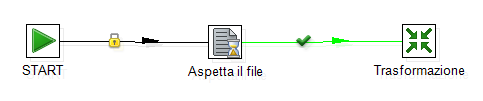
\includegraphics[scale=1]{job.png}
			\caption{\textit{Job} di trasformazione.}
			\label{fig:job}
		\end{figure}
		
		\begin{figure}[h!]
			\centering
				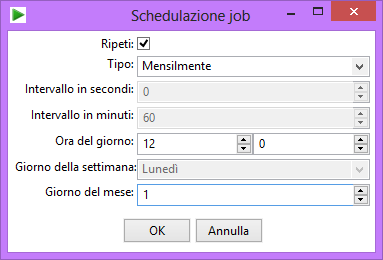
\includegraphics[scale=0.7]{job_scheduling.png}
			\caption{Impostazioni di scheduling del job.}
			\label{fig:job_scheduling}
		\end{figure}
		
		Dalla Figura \ref{fig:job} deduciamo subito la semplicità del \textit{job}: esso è formato da uno step \textit{start}, che definisce il punto di inizio e le impostazioni di scheduling, uno step di attesa, che blocca il flusso finché non è presente il \texttt{.csv} del nuovo bilancio da integrare, ed uno step \textit{trasformazione}, che è esattamente la trasformazione \textit{Kettle} precedentemente descritta in questo capitolo, opportunamente rivista per gestire un qualsiasi file di bilancio. Nella Figura \ref{fig:job_scheduling} vediamo invece il dettaglio dello step \textit{start}, dove vengono definite le impostazioni di scheduling, in modo da eseguire l'integrazione dei nuovi dati ad intervalli prefissati ed in modo del tutto automatico.\\
		\\
		In questa sezione abbiamo descritto come produrre una sorgente dati singola, dettagliata, esauriente e di alta qualità che possa alimentare il DW a partire da dati operazionali reperiti all'interno di \textit{dataset}.\\
		Le operazioni svolte, o che è possibile svolgere, tramite \textit{Kettle} sono estrazione, pulitura, trasformazione e caricamento. Nel nostro caso abbiamo semplicemente aggregato, estratto e trasformato alcune informazioni, come ad esempio la suddivisione del campo \texttt{ATTO\_DI\_IMPEGNO} o l'introduzione del nuovo campo \texttt{ANNO\_PAGAMENTO}. Non è stato necessario infatti normalizzare, standardizzare o correggere in quanto i \textit{dataset} messi a disposizione dal Comune di Firenze risultavano in quest'ottica già puliti e correttamente trasformati.\\
		Osserviamo inoltre che l'output a seguito dell'utilizzo di questo strumento può essere visto come un \textit{Refresh} per popolare il DW in un primo momento, oppure può essere interpretato come un \textit{Update} se utilizzando il \textit{job} presentato viene aggiunto alla sorgente dati finale solo il nuovo \textit{dataset} appena rilasciato.

	\chapter{Costruzione e alimentazione del Data Warehouse} \label{chap:DW}

	La tabella \texttt{Commissioni} serve per poter popolare il Data Warehouse (DW): per ogni riga di tale tabella si possono individuare le misure d'interesse, come ad esempio \texttt{IMPORTO} o \texttt{ID\_COMM}, e le dimensioni di analisi, ad esempio \texttt{BENEFICIARIO} o \texttt{ANNO\_PAGAMENTO}.\\
	Pentaho mette a disposizione uno strumento per fare \textit{On-Line Analytical Processing} (\textit{OLAP}), permettendo di creare un DW importando dati da database o da file \texttt{.csv}. Questo strumento è reso disponibile tramite un'interfaccia web, dalla quale è possibile:
	
	\begin{itemize}
	    \item importare nuovi dati sorgenti;
	    \item modificare i modelli dei dati importati;
	    \item svolgere analisi;
	    \item creare report.
	\end{itemize}
	
	È necessario fare una considerazione preliminare: l'elaborazione del file \texttt{Commissioni.csv}, realizzato nei passaggi precedenti, è computazionalmente onerosa. In uno scenario di lavoro reale il \textit{dataset} dovrebbe risiedere in un database o in una struttura ad accesso rapido. In questo lavoro è stato scelto di usare un file \texttt{.csv} per praticità e semplicità di uso, in quanto l'enfasi del progetto è rivolta verso il DW e le tecniche di analisi, piuttosto che sul relazionale.\\
	\\
	A partire dalla vista ottenuta considerando tutto il \textit{dataset} \texttt{Commissioni} possiamo creare il nostro cubo con Pentaho semplicemente selezionando a quali dimensioni e misure siamo interessati; su queste sarà poi possibile utilizzare tecniche per ridurre la quantità di dati ed ottenere informazioni utili, ad esempio per \textit{restrizione} o \textit{aggregazione}. Con \textit{restrizione} s'intende il ritagliare una porzione del cubo circoscrivendo il campo d'analisi (\textit{selezioni} e/o \textit{proiezioni}), mentre l'\textit{aggregazione} consiste nel raggruppare una o più misure rispetto ad una dimensione, ad un livello di dettaglio inferiore. Le principali \textit{funzioni d'aggregazione} utilizzate sono le seguenti:
	
	\begin{itemize}
		\item \texttt{SUM}: la misura aggregata è calcolata come somma dei singoli valori. Questa funzione viene utilizzata sul campo \texttt{IMPORTO} per calcolare costi e spese aggregate secondo certi criteri.
		\item \texttt{COUNT}: viene contato il numero di righe che hanno un valore nel campo corrispondente (da non confondere con \texttt{COUNT DISTINCT} che conta soltanto il numero di valori distinti). Questa funzione è utilizzata con il campo \texttt{ID\_COMM} per contare quante commissioni corrispondono ai criteri specificati nel filtro di query.
		\item \texttt{MAX}: la misura aggregata è il valore massimo tra quelli che corrispondono a certi criteri. Questa funzione viene utilizzata sul campo \texttt{DIFFERENZA\_PAGAMENTO\_COMMISSIONE}, in modo che venga restituita la massima differenza di anni presente per una certa Azienda.
	\end{itemize}
	
	Oltre alle funzioni sopra citate, Pentaho mette a disposizione anche \texttt{MIN}, che restituisce il minimo, e \texttt{AVERAGE}, che restituisce la media dei singoli valori.\\
	\\	
	La vista di analisi resa disponibile dalla tabella \texttt{Commissioni}, una volta selezionate le dimensioni e le misure d'interesse, è costituita da una rappresentazione navigabile del cubo \textit{OLAP} in cui è possibile fare operazioni di \textit{drill down} e \textit{drill up} sulle dimensioni stesse. Quindi la costruzione del Data Warehouse, utilizzando Pentaho, è estremamente facile. Una volta individuato il fatto d'interesse occorre solo specificare mediante un'interfaccia web quali sono le dimensioni e le misure che lo identificano e lo caratterizzano.\\
	
	\begin{figure}[h!]
		\centering
			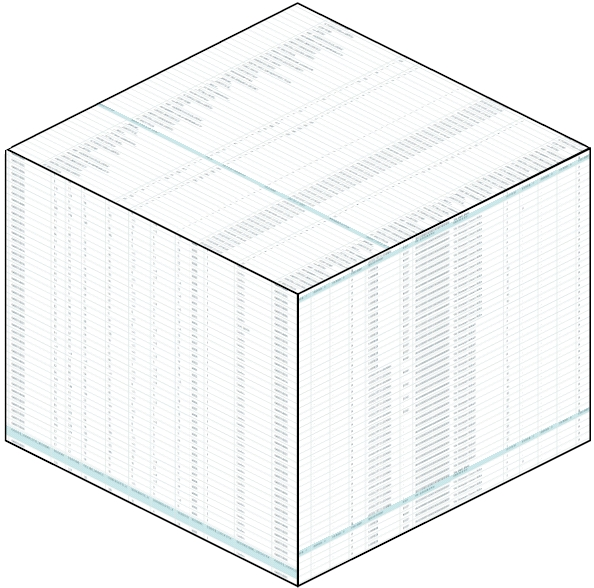
\includegraphics[scale=0.4]{cubo.jpg}
		\caption{Schema \textit{MOLAP}.}
		\label{fig:cubo1}
	\end{figure}
	
	L'alimentazione del DW consiste invece nel mantenere aggiornato il Data Warehouse nel tempo (in genere ad intervalli stabiliti). Per alimentare il Data Warehouse occorre utilizzare il \textit{job} descritto in Sezione \ref{sec:job}. Quindi dopo un primo caricamento, verrà eseguito il \textit{job} ad intervalli regolari (ad esempio ogni anno) con input il \textit{dataset} del bilancio annuale, così da inserire nel Data Warehouse dati sempre aggiornati e permettere analisi più dettagliate ed aggiornate. L'unico requisito richiesto è che i \textit{dataset} dei bilanci annuali dovranno essere già stati ripuliti e validati, così da richiedere a Pentaho di eseguire le trasformazioni necessarie per produrre una struttura compatibile con le precedenti.


	\chapter{Alcune analisi} \label{chap:analisi}
	
	In quest'ultimo capitolo ci occuperemo, finalmente, di analizzare i dati presenti nel DW costruito. Le analisi che proponiamo sono solo alcune delle possibili analisi effettuabili sui bilanci del Comune di Firenze, ma sono piuttosto significative, in quanto mostrano come, da due bilanci separati, si possano ottenere misure e considerazioni non immediate, esaltando la potenza degli strumenti di Data Warehouse.\\
	Le analisi presenti in questo capitolo saranno sia \textit{qualitative} che \textit{quantitative}: ci potremmo chiedere infatti se il Comune di Firenze ha investito o meno in un certo settore oppure quanti euro sono costati i servizi di una certa Azienda al Comune. Inoltre, alcune delle analisi qui presentate sono anche di carattere \textit{comparativo}, ovvero mettono in luce certi aspetti che intercorrono tra i due bilanci (quindi di tipo \textit{temporale}).\\
	\\
	Tutte le analisi, oltre ad una breve descrizione ed alcune considerazioni, sono costituite da un grafico (a barre o a linee) e da una tabella, che riporta i valori numerici del grafico per una miglior lettura. In alcuni casi (solitamente nelle analisi che coinvolgono aziende) sarà presente anche una tabella disaggregata, che mostrerà più nel dettaglio alcuni campi coinvolti nell'analisi. Ad esempio si mostrerà spesso in queste tabelle disaggregate il nome (o i nomi) di un'azienda associato ad una certa partita iva, per una miglior comprensione dell'analisi.
	
	\section{Totale Costi} \label{sec:costi}
		
		In questa prima sezione vedremo alcune analisi molto semplici ma significative, in quanto possono già darci un'idea delle potenzialità degli strumenti di DW, permettendoci di trarre anche le prime conclusioni.\\
		Vedremo, in particolare, alcune analisi di tipo totale che coinvolgano i pagamenti effettuati.
		
		\subsection{Confronto: Totale Costo 2012/2013} \label{subsec:costi}
			
			La prima di queste analisi consiste in un confronto tra il costo totale (calcolato come \texttt{pagamenti+crediti}) dell'anno 2012 e del 2013.\\
			
			\begin{figure}[h!]
				\centering
					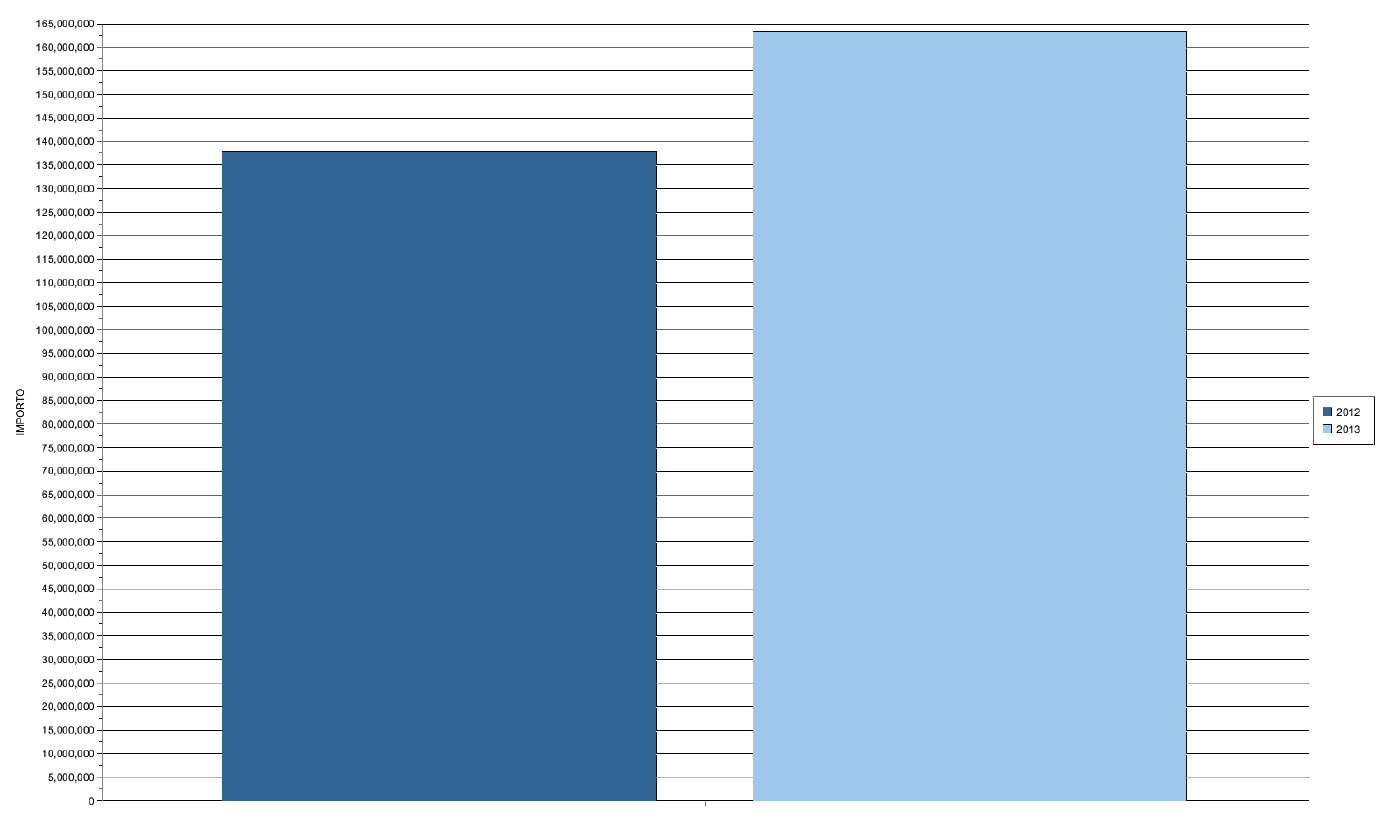
\includegraphics[scale=0.5]{totale_costo.png}
				\caption{Totale Costo 2012/2013, grafico.}
				\label{fig:totale_costo}
			\end{figure}
			
			\begin{figure}[h!]
				\centering
					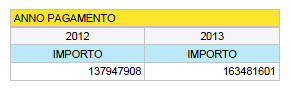
\includegraphics[scale=0.8]{totale_costo_tab.png}
				\caption{Totale Costo 2012/2013, tabella.}
				\label{fig:totale_costo_tab}
			\end{figure}
			
			Nonostante il bilancio 2013 non sia definitivo, vediamo come quest'ultimo superi già il bilancio 2012 in termini di costo di circa 25 milioni di euro. Questa disparità può essere spiegata col fatto che il bilancio 2012 è, a sua volta, non completo, in quanto, come già accennato nel Capitolo \ref{chap:elaborazione}, esso inizia a partire dal 26 giugno 2012.
			
			\FloatBarrier
			
		\subsection{Confronto: Totale Pagamenti/Crediti 2012/2013} \label{subsce:pagamenti/crediti}
		
			In questa analisi partiamo dalla precedente ed entriamo nel dettaglio di Pagamenti e Crediti, disaggregando rispetto al campo \texttt{DOCUMENTO}, che indica se una commissione è una \textit{fattura} o una \textit{nota di credito}.\\
			
			\begin{figure}[h!]
				\centering
					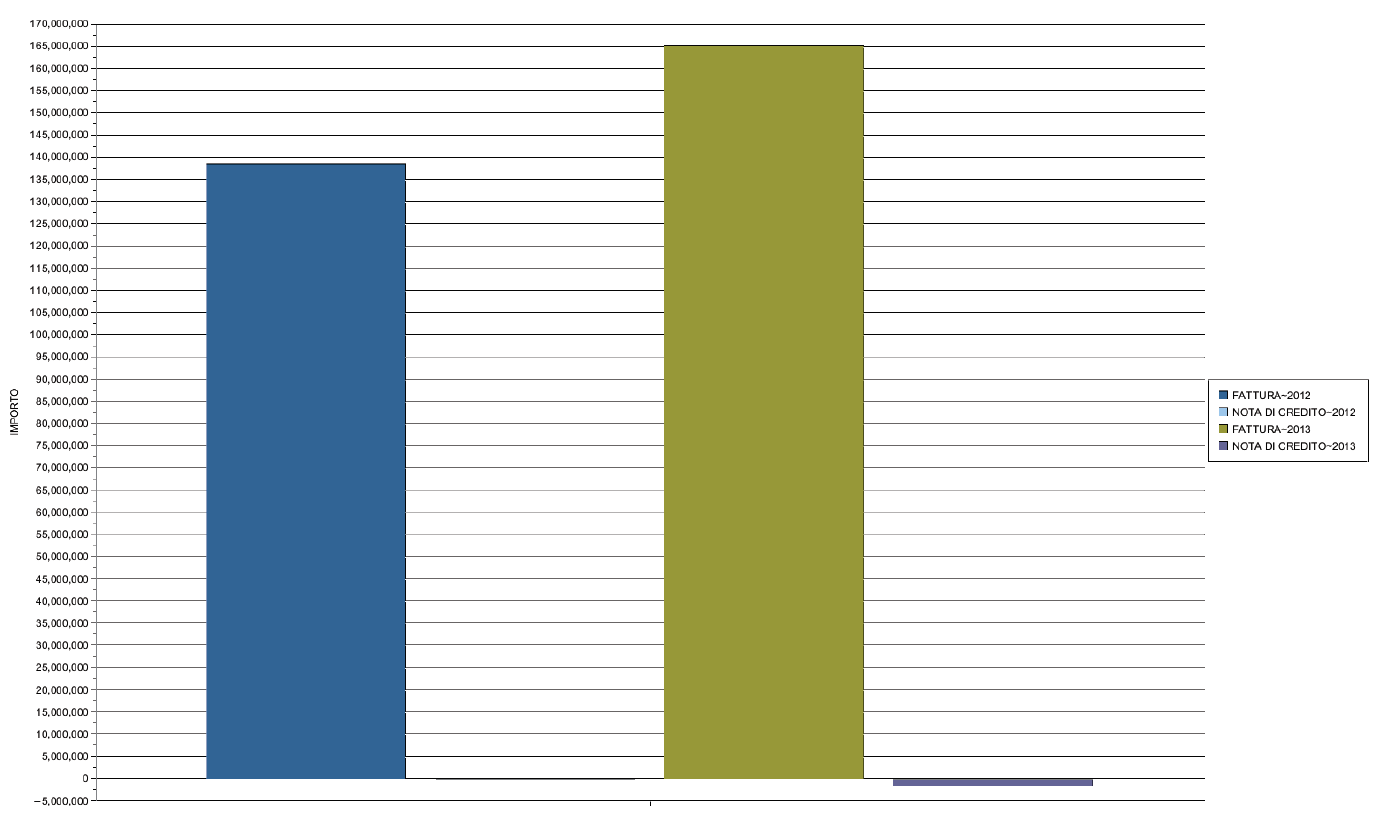
\includegraphics[scale=0.5]{totale_pagamenti-crediti.png}
				\caption{Totale Pagamenti/Crediti 2012/2013, grafico.}
				\label{fig:totale_pagamenti-crediti}
			\end{figure}
			
			\begin{figure}[h!]
				\centering
					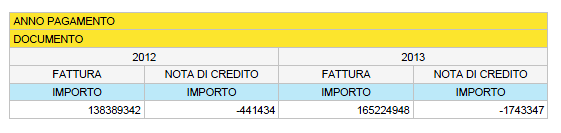
\includegraphics[scale=0.8]{totale_pagamenti-crediti_tab.png}
				\caption{Totale Pagamenti/Crediti 2012/2013, tabella.}
				\label{fig:totale_pagamenti-crediti_tab}
			\end{figure}
			
			Come nel caso precedente, notiamo che il bilancio 2013 presenta valori più alti (in valore assoluto), sia per Pagamenti che per Crediti, probabilmente per la stessa considerazione fatta precedentemente.
			
			\FloatBarrier
			
		\subsection{Confronto: Totale Fatture/Note di Credito 2012/2013} \label{subsec:fatture/notedicredito}
		
			Per avere una conferma delle supposizioni fatte nelle ultime due analisi, andiamo ad osservare quanti mandati sono stati commissionati negli anni 2012/2013, mantenendo la distinzione tra fatture e note di credito.\\
		
			\begin{figure}[h!]
				\centering
					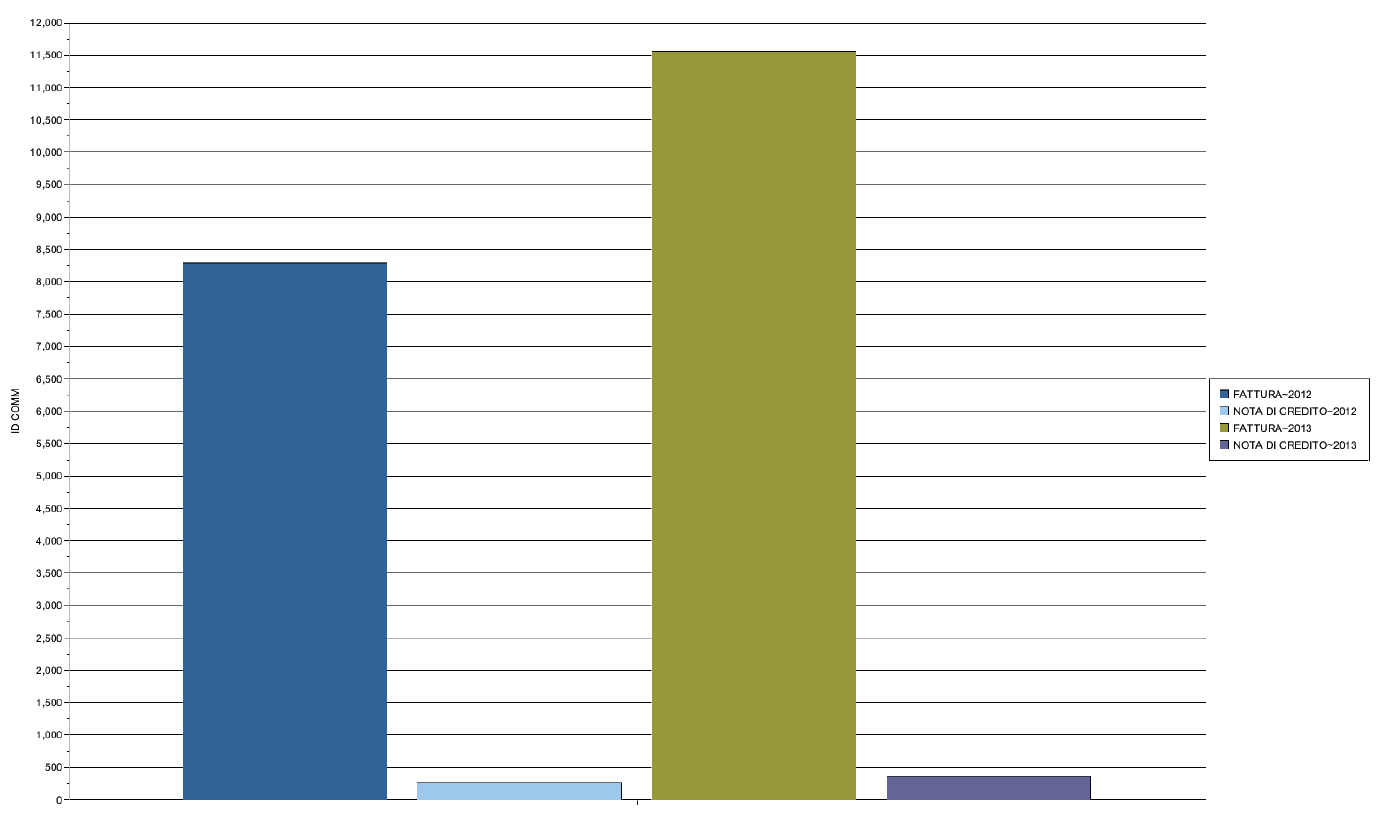
\includegraphics[scale=0.5]{totale_fatture-notedicredito.png}
				\caption{Totale Fatture/Note di Credito 2012/2013, grafico.}
				\label{fig:totale_fatture-notedicredito}
			\end{figure}
			
			\begin{figure}[h!]
				\centering
					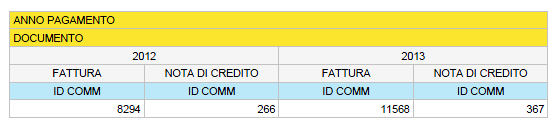
\includegraphics[scale=0.8]{totale_fatture-notedicredito_tab.png}
				\caption{Totale Fatture/Note di Credito 2012/2013, tabella.}
				\label{fig:totale_fatture-notedicredito_tab}
			\end{figure}
			
			Come ci aspettavamo, si nota che nel 2013 sono stati commissionati più lavori (sia a credito che non), probabilmente proprio a causa delle mancanze presenti nel bilancio 2012 prima menzionate.
			
			\FloatBarrier
			
	\section{TOP 10 Pagamenti per Aziende} \label{sec:pagamenti_aziende}
		
		Le analisi di questa sezione saranno orientate ad individuare le Aziende più pagate dal Comune di Firenze: vedremo innanzitutto la Top-10 delle Aziende più pagate nel 2012, quindi nel 2013 ed infine verrano confrontati i pagamenti tra 2012 e 2013 per le Aziende relative alla prima di queste analisi.
		
		\subsection{TOP 10 Pagamenti per Aziende 2012} \label{subsec:pagamenti_aziende_2012}
		
			Vediamo in questa analisi quali sono state le 10 Aziende più pagate dal Comune di Firenze durante l'anno 2012.\\
			
			\begin{figure}[h!]
				\centering
					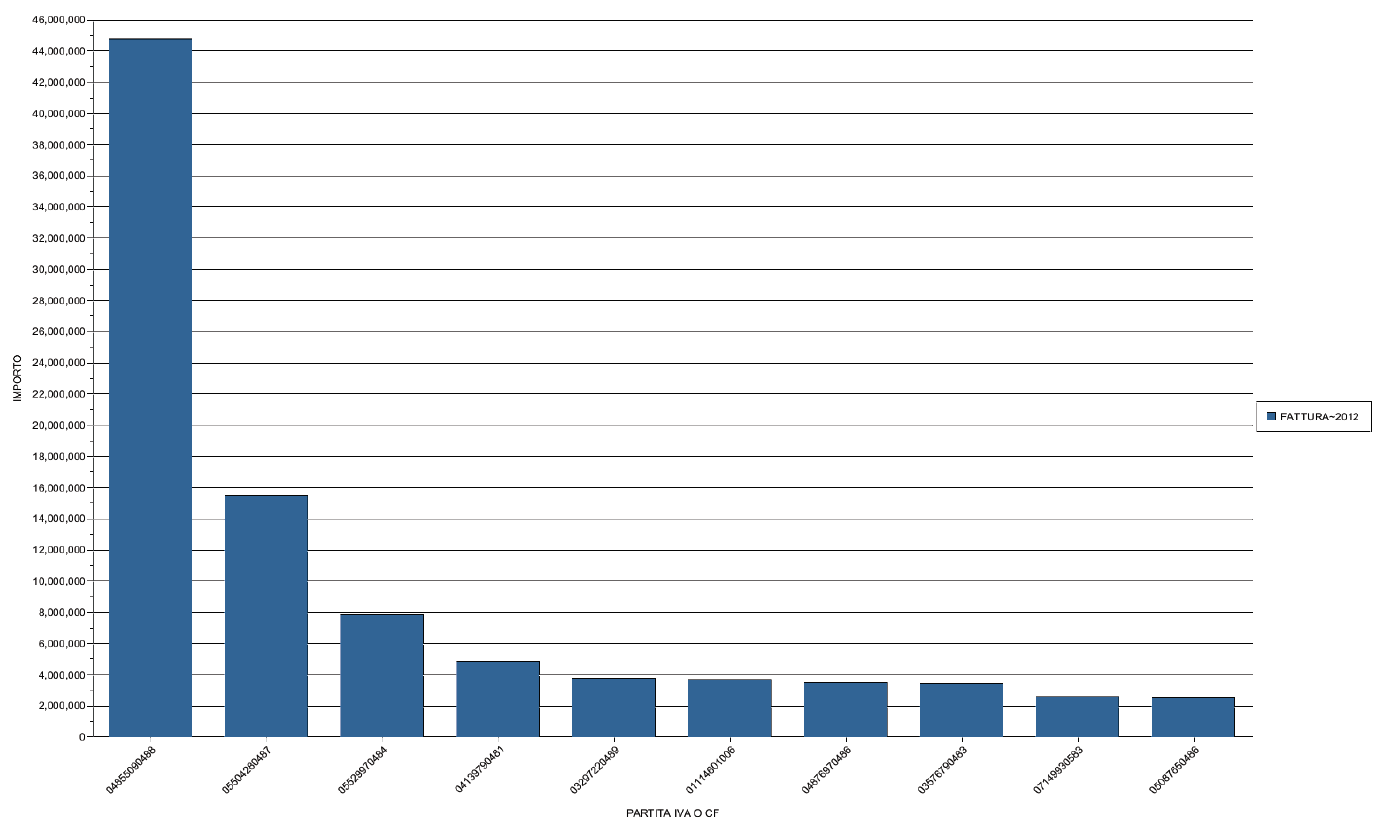
\includegraphics[scale=0.5]{top10_pagamenti_aziende_2012.png}
				\caption{TOP 10 Pagamenti per Aziende 2012, grafico.}
				\label{fig:top10_pagamenti_aziende_2012}
			\end{figure}
			
			\begin{figure}[h!]
				\centering
					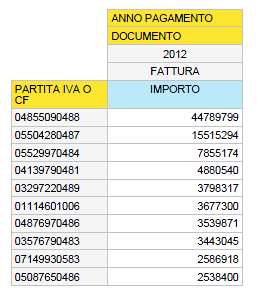
\includegraphics[scale=0.8]{top10_pagamenti_aziende_2012_tab.png}
				\caption{TOP 10 Pagamenti per Aziende 2012, tabella.}
				\label{fig:top10_pagamenti_aziende_2012_tab}
			\end{figure}
			
			\begin{figure}[h!]
				\centering
					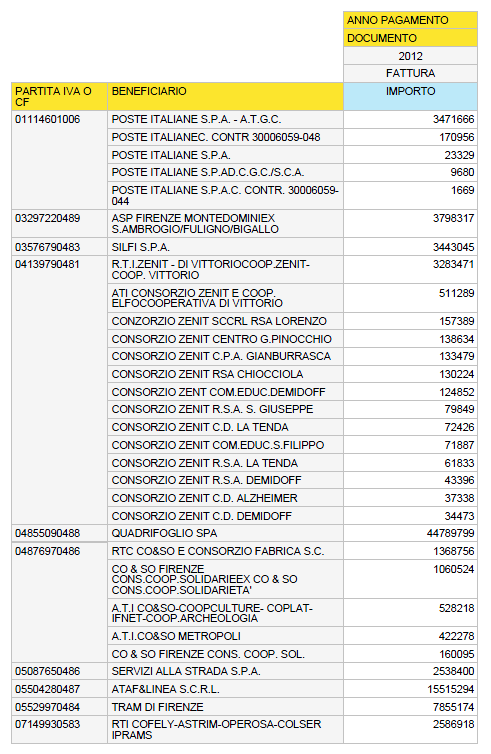
\includegraphics[scale=0.8]{top10_pagamenti_aziende_2012_tab_dis.png}
				\caption{TOP 10 Pagamenti per Aziende 2012, tabella disaggregata.}
				\label{fig:top10_pagamenti_aziende_2012_tab_dis}
			\end{figure}
			
			Si nota subito l'enorme disparità che intercorre tra la prima Azienda, ovvero la \textit{Quadrifoglio s.p.a.}, e tutte le altre presenti nella Top-10.\\
			La \textit{Quadrifoglio s.p.a.} è un'Azienda di Firenze che si occupa di servizi ambientali nel Comune di Firenze e nei comuni limitrofi, offrendo servizi come raccolta e smaltimento rifiuti, in primo luogo, ma anche come disinfestazione (zanzare, topi, ecc\dots) o centro di analisi e ricerca. È quindi un'Azienda molto importante, ormai onnipresente nell'ambiente fiorentino, che giustifica tutte le spese osservate.\\
			Com'è facile aspettarsi, al secondo e terzo posto troviamo altre due Aziende onnipresenti nello senario fiorentino: \textit{ATAF\&Linea S.C.R.L.} e \textit{Tram di Firenze}, che si occupano, rispettivamente, del servizio di autobus e della tramvia fiorentina.
			Tra le altre Aziende, troviamo altri nomi ben conosciuti come \textit{Consorzio Zenit}, che si occupa di interventi educativi, formativi e sanitari, e le \textit{Poste Italiane}.
			
			\FloatBarrier
		
		\subsection{TOP 10 Pagamenti per Aziende 2013} \label{subsec:pagamenti_aziende_2013}
		
			Ripetiamo qui l'analisi precedente sull'anno 2013 anziché 2012.\\
		
			\begin{figure}[h!]
				\centering
					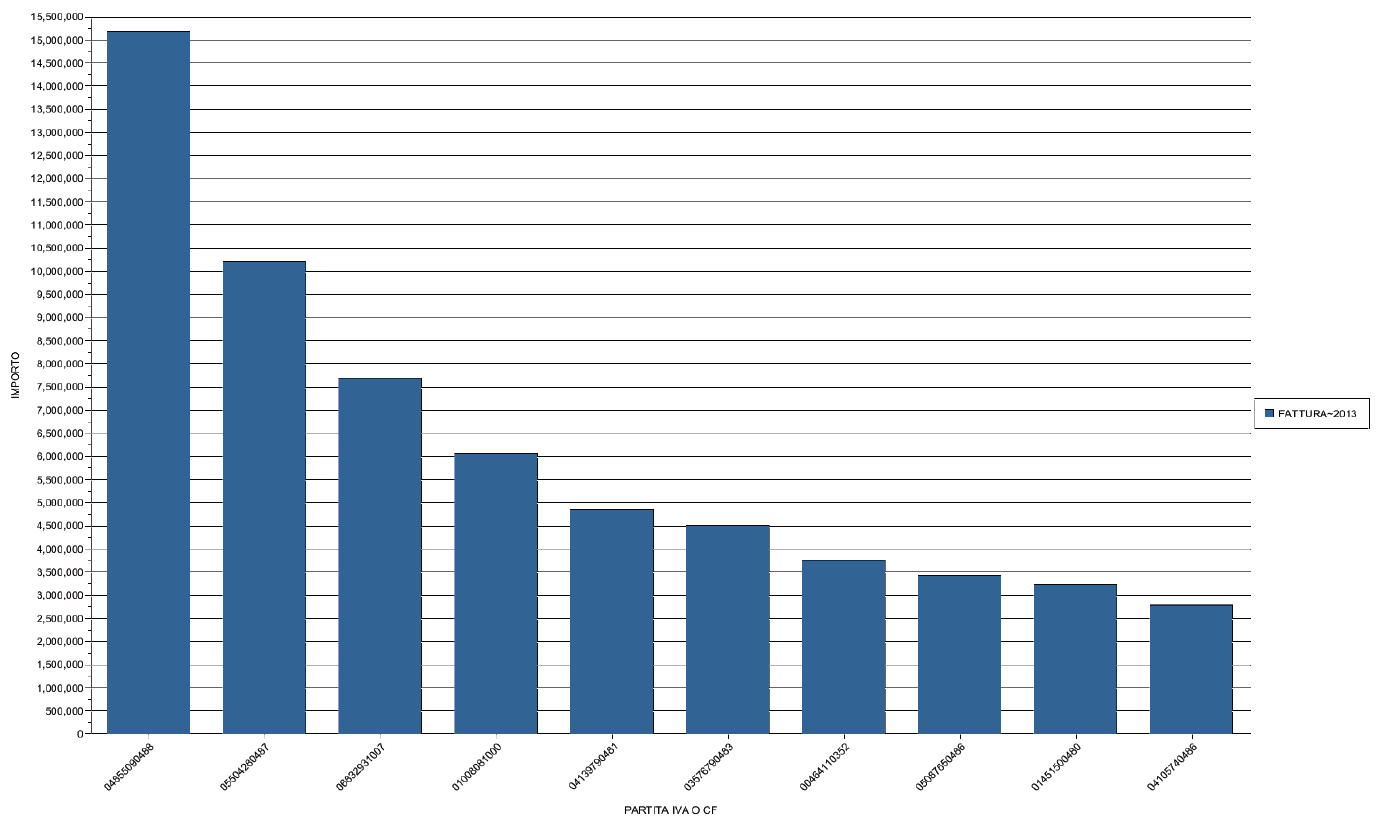
\includegraphics[scale=0.5]{top10_pagamenti_aziende_2013.png}
				\caption{TOP 10 Pagamenti per Aziende 2013, grafico.}
				\label{fig:top10_pagamenti_aziende_2013}
			\end{figure}
			
			\begin{figure}[h!]
				\centering
					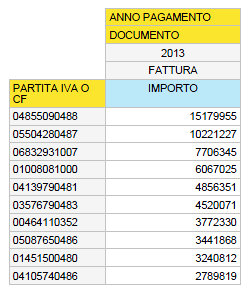
\includegraphics[scale=0.8]{top10_pagamenti_aziende_2013_tab.png}
				\caption{TOP 10 Pagamenti per Aziende 2013, tabella.}
				\label{fig:top10_pagamenti_aziende_2013_tab}
			\end{figure}
			
			\begin{figure}[h!]
				\centering
					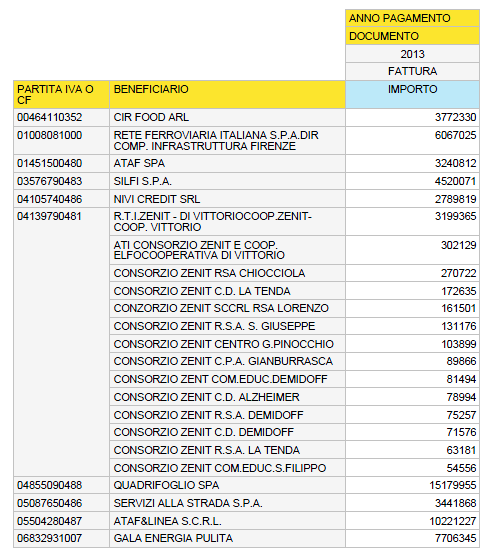
\includegraphics[scale=0.8]{top10_pagamenti_aziende_2013_tab_dis.png}
				\caption{TOP 10 Pagamenti per Aziende 2013, tabella disaggregata.}
				\label{fig:top10_pagamenti_aziende_2013_tab_dis}
			\end{figure}
			
			Al primo e secondo posto troviamo ancora la \textit{Quadrifoglio s.p.a.} e \textit{ATAF\&Linea S.C.R.L.}, esattamente come nel 2012. Al terzo posto troviamo invece \textit{Gala Energia Pulita}, che si occupa di fornitura energetica. Tra le altre, ritroviamo il \textit{Consorzio Zenit} ed altre Aziende.
			
			\FloatBarrier
		
		\subsection{Confronto: TOP 10 Pagamenti per Aziende 2012/2013} \label{subsec:pagamenti_aziende_2012/2013}
	
			Vediamo adesso come le Aziende presenti nella Top-10 di Pagamenti del 2012 vengono pagate tra il 2012 ed il 2013.\\
	
			\begin{figure}[h!]
				\centering
					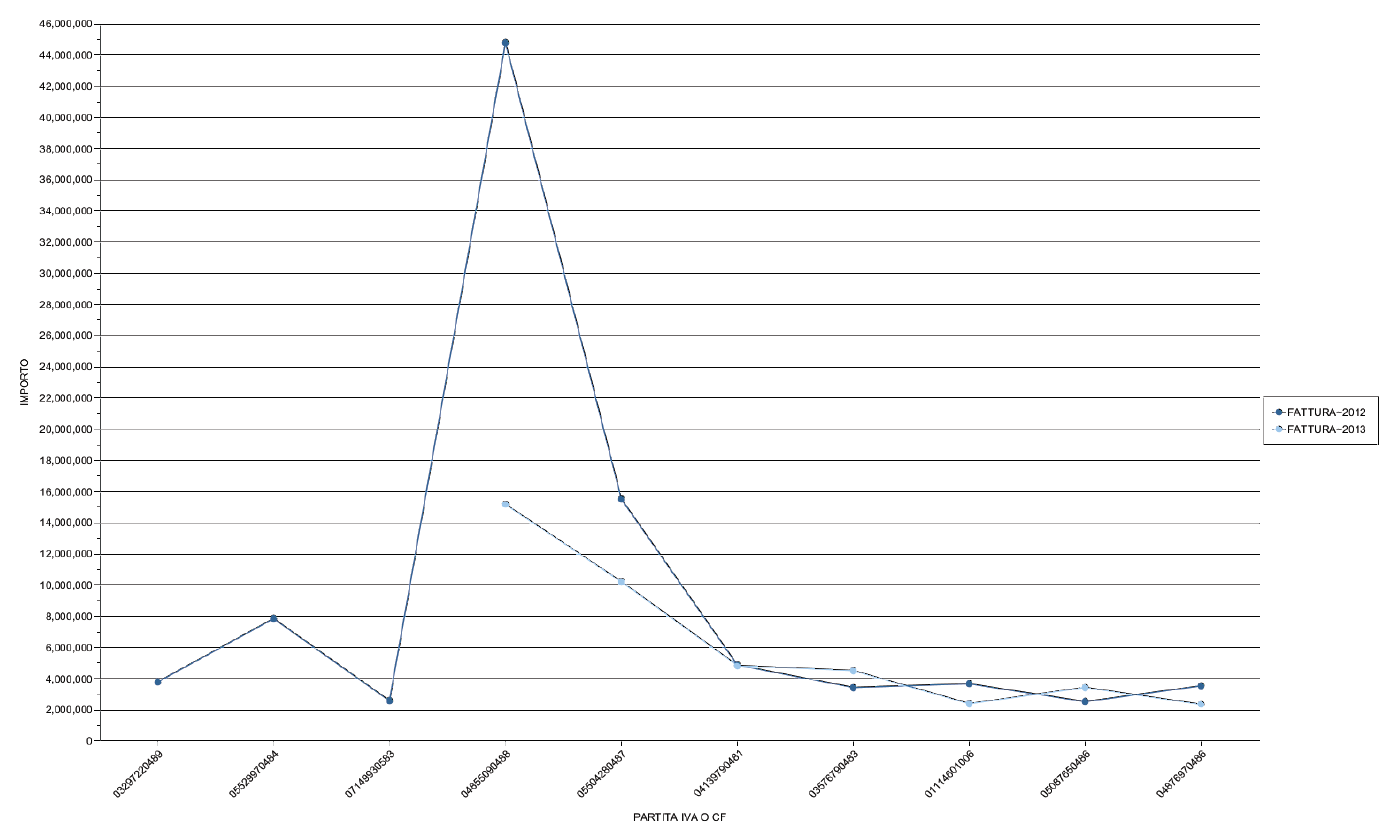
\includegraphics[scale=0.5]{top10_pagamenti_aziende_2012-2013.png}
				\caption{TOP 10 Pagamenti per Aziende 2012/2013, grafico.}
				\label{fig:top10_pagamenti_aziende_2012-2013}
			\end{figure}
			
			\begin{figure}[h!]
				\centering
					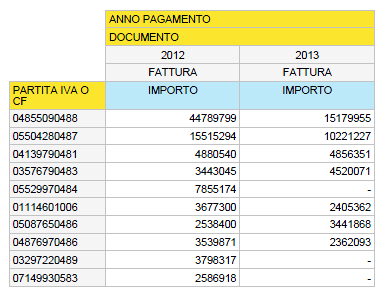
\includegraphics[scale=0.8]{top10_pagamenti_aziende_2012-2013_tab.png}
				\caption{TOP 10 Pagamenti per Aziende 2012/2013, tabella.}
				\label{fig:top10_pagamenti_aziende_2012-2013_tab}
			\end{figure}
			
			\begin{figure}[h!]
				\centering
					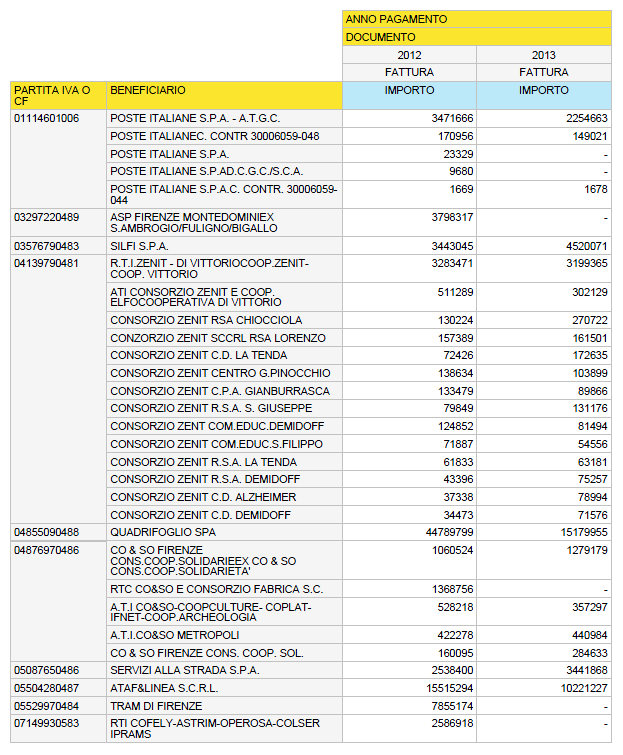
\includegraphics[scale=0.8]{top10_pagamenti_aziende_2012-2013_tab_dis.png}
				\caption{TOP 10 Pagamenti per Aziende 2012/2013, tabella disaggregata.}
				\label{fig:top10_pagamenti_aziende_2012-2013_tab_dis}
			\end{figure}
			
			Si notano innanzitutto tre aziende (\textit{Tram di Firenze}, \textit{RTI Cofely-Astrim-Operosa-Colser Iprams} e \textit{ASP Firenze Montedomini}) presenti nella Top-10 2012 e del tutto assenti nel bilancio 2013, indice, probabilmente, di Aziende a cui erano stati assegnati lavori una tantum. Si nota inoltre la disparità dei pagamenti verso \textit{Quadrifoglio s.p.a.} che, nonostante sia comunque la più pagata delle Aziende, ha registrato comunque un forte crollo rispetto al 2012. Per quanto riguarda le altre Aziende, si registra invece un andamento piuttosto regolare nel biennio 2012/2013.
			
			\FloatBarrier
	
	\section{TOP 10 Pagamenti per Direzioni} \label{sec:top_pagamenti_direzioni}
	
		Dal momento che le Direzioni di Servizio sono delle classificazioni per area di competenza del Comune di Firenze, possiamo vedere i pagamenti approvati da una certa Direzione come gli investimenti del Comune nelle rispettive aree.\\
		\\
		Eseguiamo in questa sezione le stesse analisi effettuate in Sezione \ref{sec:pagamenti_aziende}, con l'unica differenza che i pagamenti saranno aggregati per Direzione di Servizio e non più per Azienda. Potremo analizzare in questo modo in quali aree ha scelto di investire il Comune di Firenze e come queste scelte si siano evolute tra il 2012 ed il 2013.
	
		\subsection{TOP 10 Pagamenti per Direzioni 2012} \label{subsec:top_pagamenti_direzioni_2012}
		
			La prima analisi da effettuare è relativa alle 10 Direzioni di Servizio che, nel 2012, hanno pagato di più rispetto alle altre.
		
			\begin{figure}[h!]
				\centering
					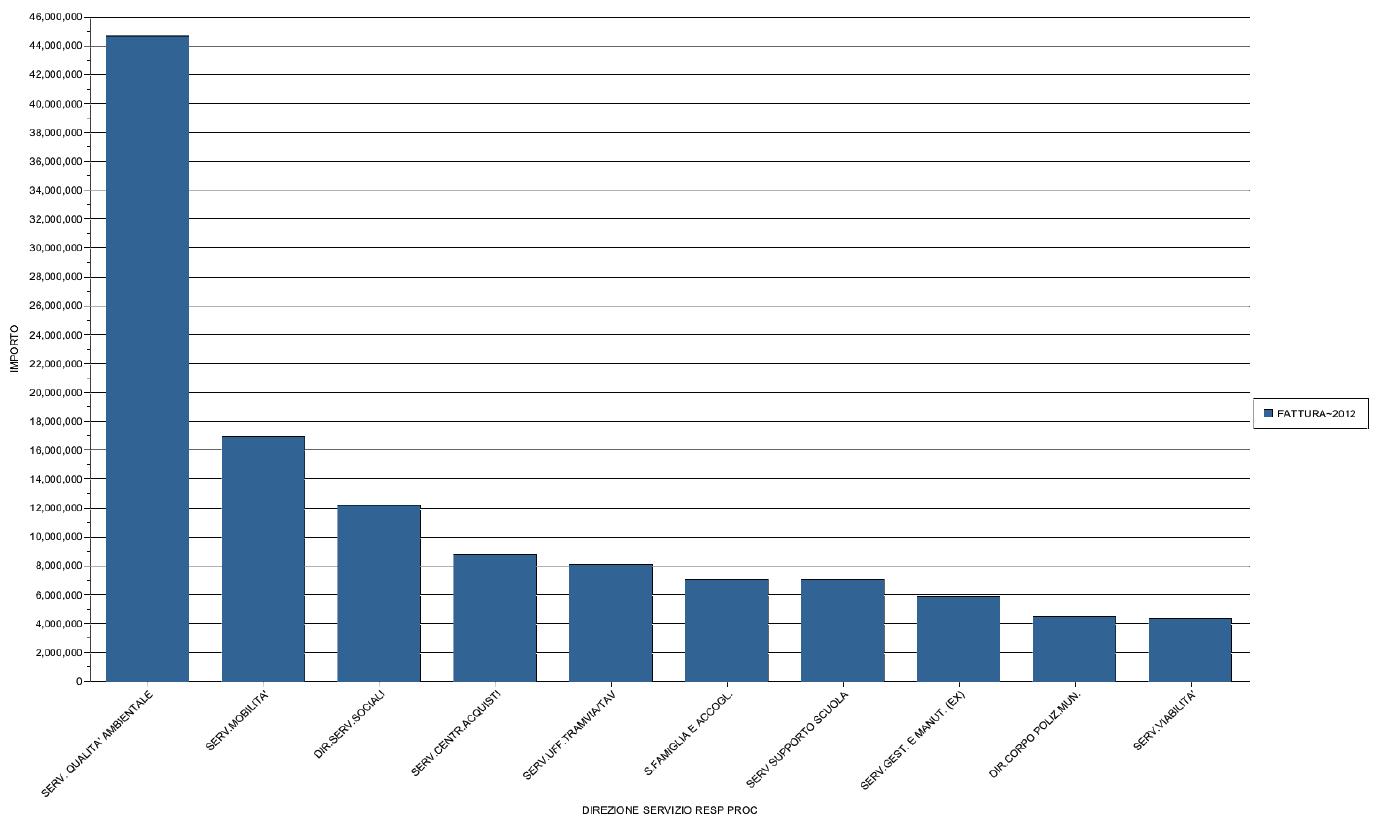
\includegraphics[scale=0.5]{top10_pagamenti_direzioni_2012.png}
				\caption{TOP 10 Pagamenti per Direzioni 2012, grafico.}
				\label{fig:top10_pagamenti_direzioni_2012}
			\end{figure}
			
			\begin{figure}[h!]
				\centering
					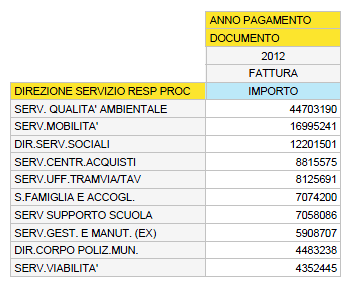
\includegraphics[scale=0.8]{top10_pagamenti_direzioni_2012_tab.png}
				\caption{TOP 10 Pagamenti per Direzioni 2012, tabella.}
				\label{fig:top10_pagamenti_direzioni_2012_tab}
			\end{figure}
			
			Come era intuibile, le Direzioni ad aver speso di più nel 2012 sono \textit{Servizi Qualità Ambientale} e \textit{Servizi Mobilità} (ricordando dalle analisi in Sezione \ref{sec:pagamenti_aziende} che le aziende più pagate nel 2012 erano la \textit{Quadrifoglio s.p.a.}, \textit{Ataf} e \textit{Tram di Firenze}). Tra le altre Direzioni presenti nella Top-10 troviamo altri settori molto importanti, come \textit{Servizi Supporto Scuola}, \textit{Direzione Corpo Polizia Municipale} e \textit{Servizi Viabilità}.
			
			\FloatBarrier
		
		\subsection{TOP 10 Pagamenti per Direzioni 2013} \label{subsec:top_pagamenti_direzioni_2013}
		
			Ripetiamo adesso le analisi per l'anno 2013.
			
			\begin{figure}[h!]
				\centering
					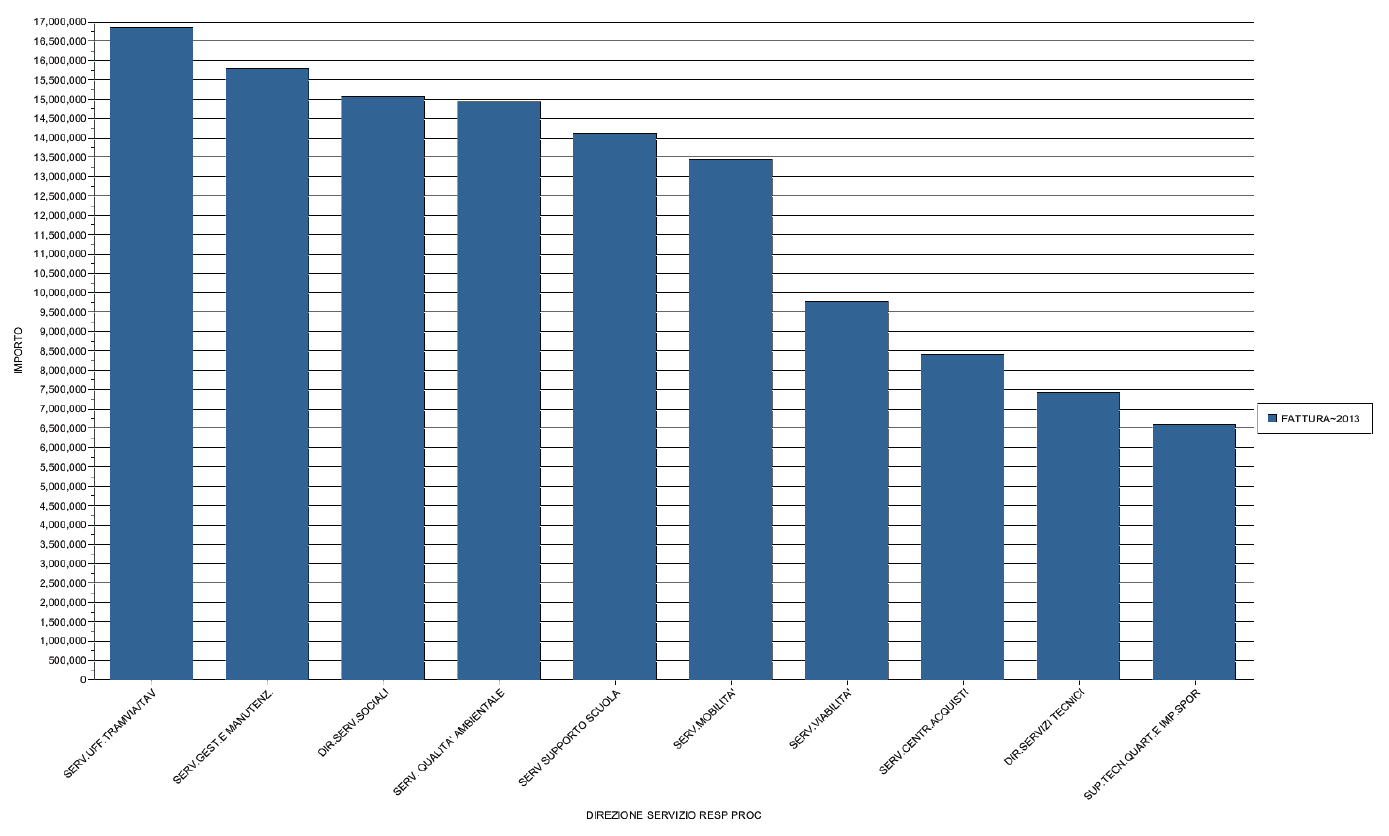
\includegraphics[scale=0.5]{top10_pagamenti_direzioni_2013.png}
				\caption{TOP 10 Pagamenti per Direzioni 2013, grafico.}
				\label{fig:top10_pagamenti_direzioni_2013}
			\end{figure}
			
			\begin{figure}[h!]
				\centering
					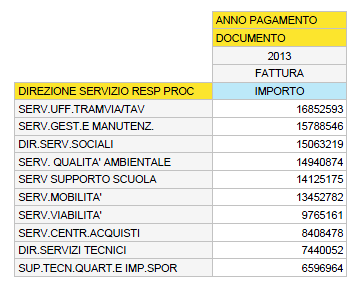
\includegraphics[scale=0.8]{top10_pagamenti_direzioni_2013_tab.png}
				\caption{TOP 10 Pagamenti per Direzioni 2013, tabella.}
				\label{fig:top10_pagamenti_direzioni_2013_tab}
			\end{figure}
			
			Vediamo in questo grafico (Figura \ref{fig:top10_pagamenti_direzioni_2013} che gli importi pagati dalle prima 10 Direzioni nel 2013 sono piuttosto regolari, senza sbalzi o irregolarità troppo evidenti. Rispetto al 2012, gli investimenti sono stati indirizzati più o meno nelle stesse direzioni.
			
			\FloatBarrier
		
		\subsection{Confronto: TOP 10 Pagamenti per Direzioni 2012/2013} \label{subsec:pagamenti_direzioni_2012/2013}
	
			Confrontiamo adesso le Direzioni con più investimenti nel 2012 con gli investimenti nel 2013 (relativamente alle stesse Direzioni di Servizio).
	
			\begin{figure}[h!]
				\centering
					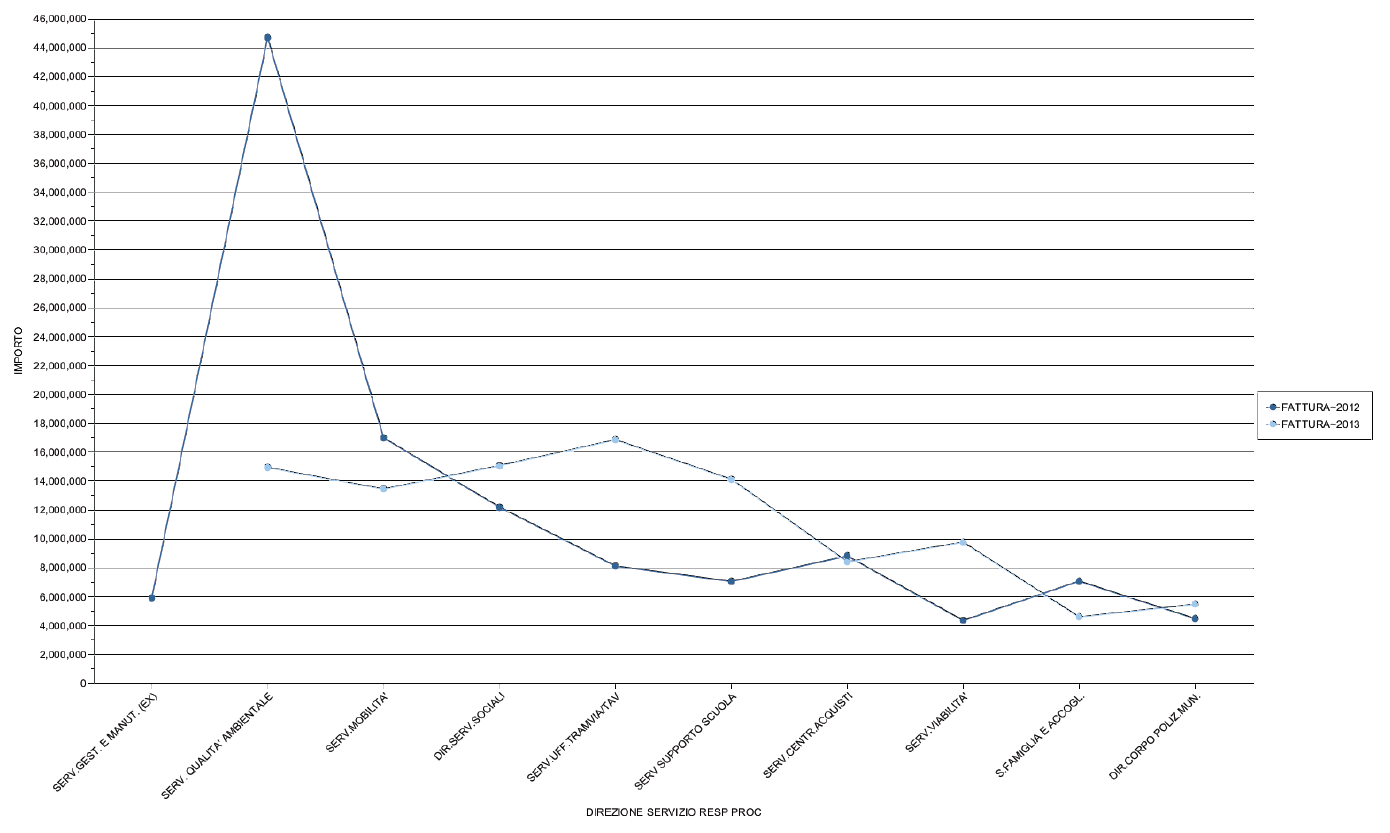
\includegraphics[scale=0.5]{top10_pagamenti_direzioni_2012-2013.png}
				\caption{TOP 10 Pagamenti per Direzioni 2012/2013, grafico.}
				\label{fig:top10_pagamenti_direzioni_2012-2013}
			\end{figure}
			
			\begin{figure}[h!]
				\centering
					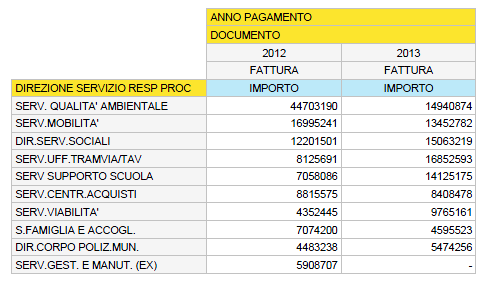
\includegraphics[scale=0.8]{top10_pagamenti_direzioni_2012-2013_tab.png}
				\caption{TOP 10 Pagamenti per Direzioni 2012/2013, tabella.}
				\label{fig:top10_pagamenti_direzioni_2012-2013_tab}
			\end{figure}
			
			A parte \textit{Servizi Gestione e Manutenzione}, che non è presente nel bilancio 2013, notiamo nel grafico in Figura \ref{fig:top10_pagamenti_direzioni_2012-2013} un netto distacco nei finanziamenti 2012 e 2013. Il cambiamento più eclatante risulta essere quello relativo ai \textit{Servizi Qualità Ambientale}, in accordo con quanto osservato in Sezione \ref{sec:pagamenti_aziende}, che registra un calo di quasi 30 milioni di euro negli investimenti, pari a circa $66\%$ degli investimenti registrati nel 2012.
			
			\FloatBarrier
	
	\section{BOTTOM 10 Pagamenti per Direzioni} \label{sec:bottom_pagamenti_direzioni}
	
		Avendo osservato le Direzioni con più investimenti, analizziamo in questa sezione le aree con meno investimenti.
	
		\subsection{BOTTOM 10 Pagamenti per Direzioni 2012} \label{subsec:bottom_pagamenti_direzioni_2012}
		
			Questa analisi rappresenta la Bottom-10 degli investimenti nel 2012, ovvero le 10 Direzioni di Servizio del Comune di Firenze che hanno speso meno nell'anno 2012.
		
			\begin{figure}[h!]
				\centering
					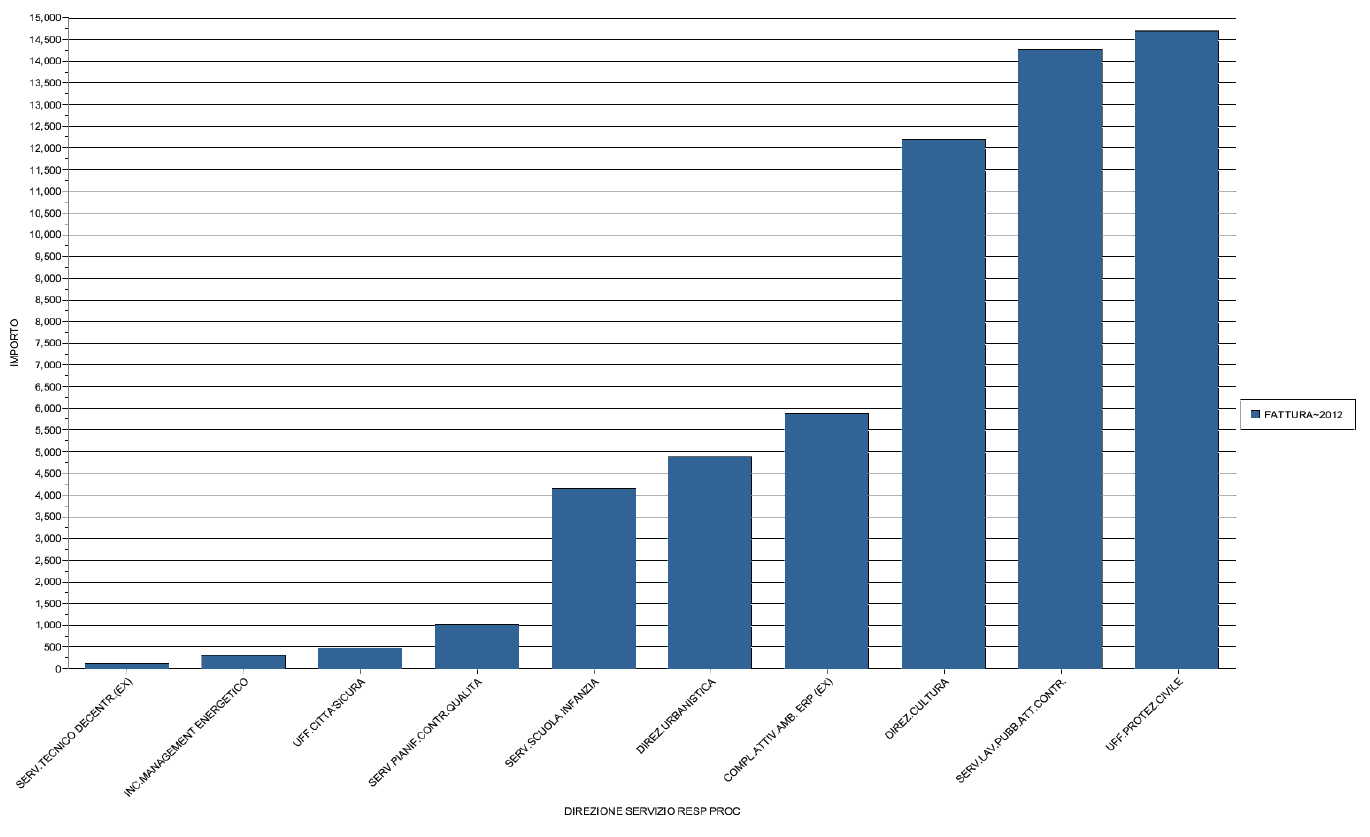
\includegraphics[scale=0.5]{bottom10_pagamenti_direzioni_2012.png}
				\caption{BOTTOM 10 Pagamenti per Direzioni 2012, grafico.}
				\label{fig:bottom10_pagamenti_direzioni_2012}
			\end{figure}
			
			\begin{figure}[h!]
				\centering
					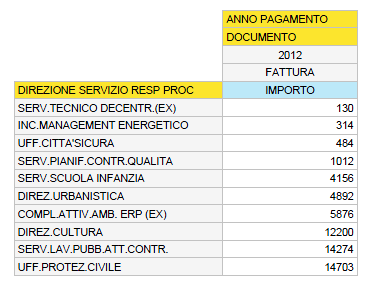
\includegraphics[scale=0.8]{bottom10_pagamenti_direzioni_2012_tab.png}
				\caption{BOTTOM 10 Pagamenti per Direzioni 2012, tabella.}
				\label{fig:bottom10_pagamenti_direzioni_2012_tab}
			\end{figure}
			
			Osservando il grafico di quest'analisi, si può vedere come alcuni importanti settori, come \textit{Protezione Civile}, \textit{Cultura} o \textit{Scuola dell'Infanzia}, siano stati alquanto trascurate per quanto riguarda gli investimenti promossi dal Comune di Firenze. Anche se si tratta, senza dubbio, di aree molto importanti, quella con più investimenti tra le 10 in questione registra poco più di 14mila euro di investimenti, mentre la prima registra soltanto 130 euro.
			
			\FloatBarrier
		
		\subsection{BOTTOM 10 Pagamenti per Direzioni 2013} \label{subsec:bottom_pagamenti_direzioni_2013}
		
			Analizziamo adesso gli investimenti più bassi nel 2013.
		
			\begin{figure}[h!]
				\centering
					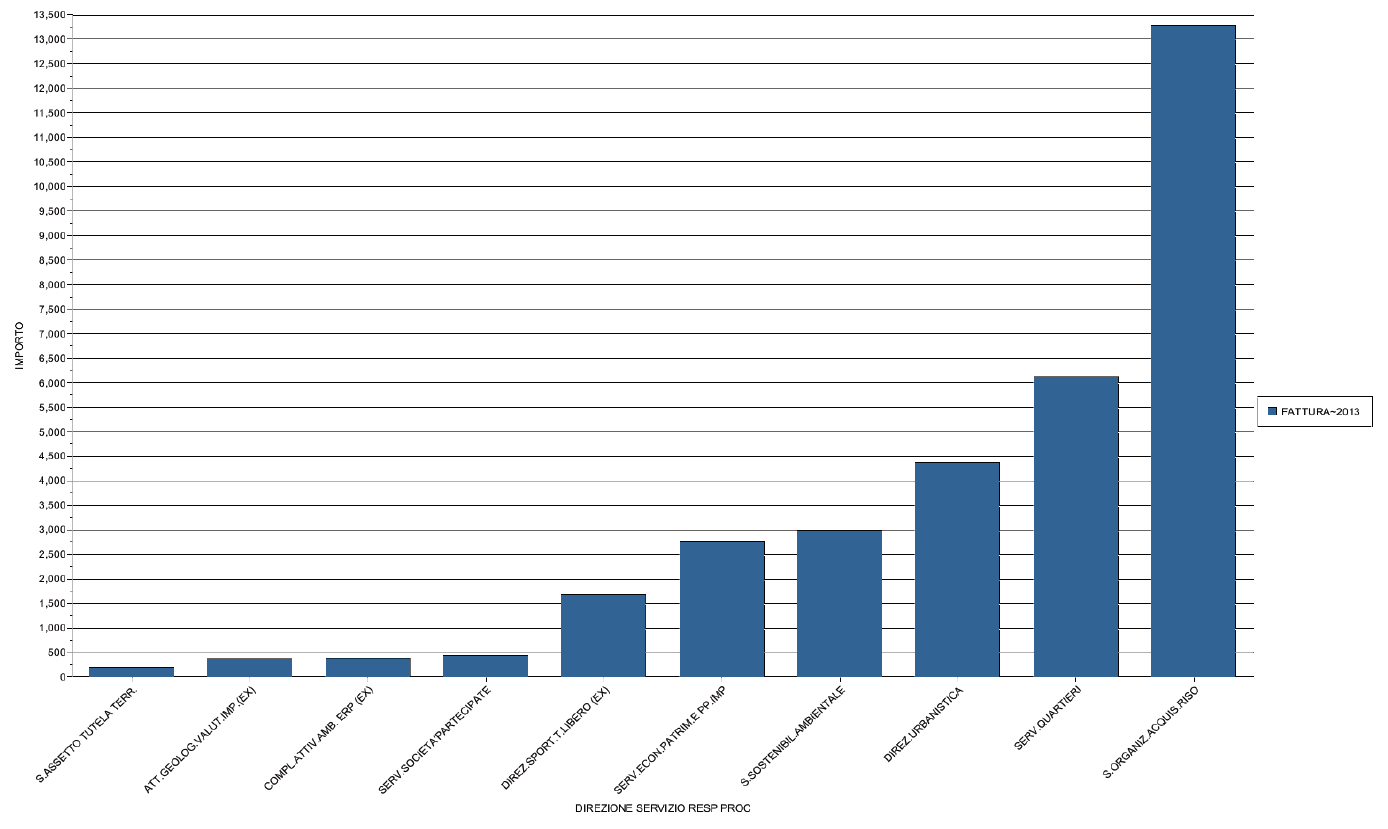
\includegraphics[scale=0.5]{bottom10_pagamenti_direzioni_2013.png}
				\caption{BOTTOM 10 Pagamenti per Direzioni 2013, grafico.}
				\label{fig:bottom10_pagamenti_direzioni_2013}
			\end{figure}
			
			\begin{figure}[h!]
				\centering
					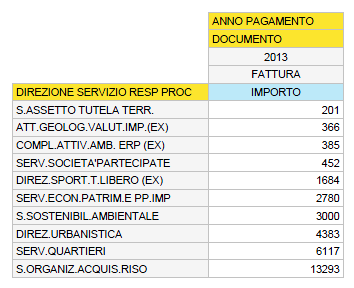
\includegraphics[scale=0.8]{bottom10_pagamenti_direzioni_2013_tab.png}
				\caption{BOTTOM 10 Pagamenti per Direzioni 2013, tabella.}
				\label{fig:bottom10_pagamenti_direzioni_2013_tab}
			\end{figure}
			
			Fortunatamente, dal grafico e dalla tabella risulta che durante il 2013 gli investimenti più bassi del Comune di Firenze sono relativi a settori ed aree minori, che giustificano i bassi costi riscontrati.
			
			\FloatBarrier
		
		\subsection{Confronto: BOTTOM 10 Pagamenti per Direzioni 2012/2013} \label{subsec:bottom_pagamenti_direzioni_2012/2013}
	
			Confrontiamo adesso le Direzioni che hanno pagato di meno nel 2012, mostrando la loro evoluzione tra il 2012 ed il 2013.
	
			\begin{figure}[h!]
				\centering
					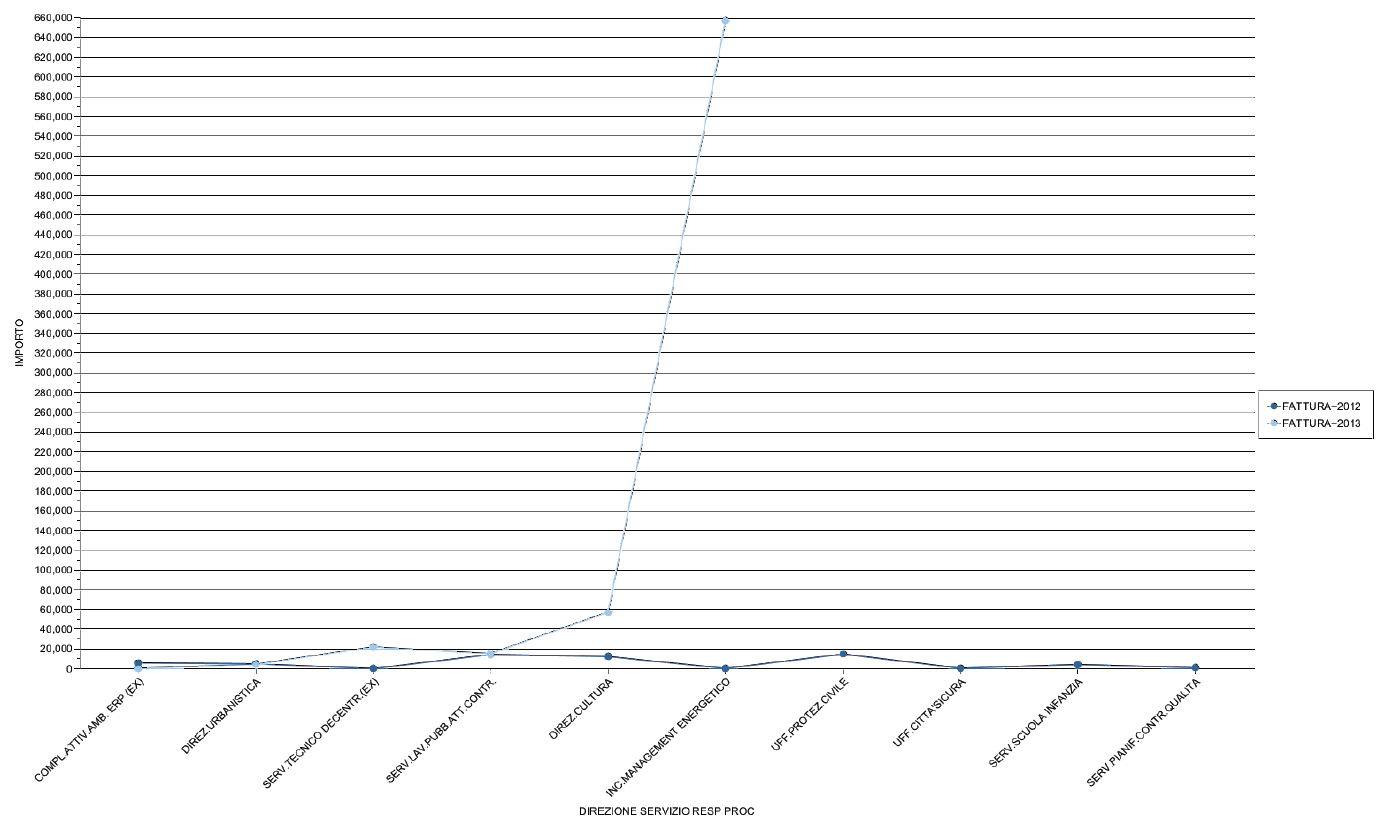
\includegraphics[scale=0.5]{bottom10_pagamenti_direzioni_2012-2013.png}
				\caption{BOTTOM 10 Pagamenti per Direzioni 2012/2013, grafico.}
				\label{fig:bottom10_pagamenti_direzioni_2012-2013}
			\end{figure}
			
			\begin{figure}[h!]
				\centering
					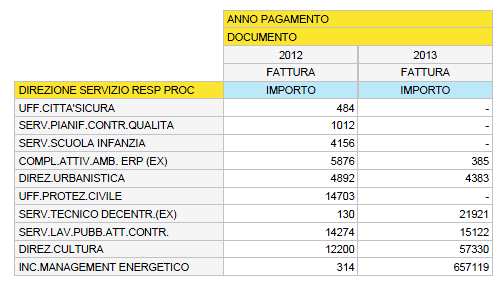
\includegraphics[scale=0.8]{bottom10_pagamenti_direzioni_2012-2013_tab.png}
				\caption{BOTTOM 10 Pagamenti per Direzioni 2012/2013, tabella.}
				\label{fig:bottom10_pagamenti_direzioni_2012-2013_tab}
			\end{figure}
			
			La cosa che risalta subito all'occhio è l'enorme distacco presente negli investimenti nel settore \textit{Management Energetico}, che registra un sostanziale aumento di finanziamenti nel 2013 rispetto al 2012. Inoltre si nota anche un aumento degli investimenti di circa il $369\%$ per quanto riguarda il settore della \textit{Cultura}.\\
			Per quanto riguarda le altre Direzioni, o esse sono assenti nel bilancio 2013, o gli investimenti risultano essere più o meno gli stessi del 2012.
			
			\FloatBarrier
	
	\section{TOP 10 Accoppiate Direzione-Azienda} \label{sec:accoppiate}
		
		Proponiamo in questa sezione un'analisi piuttosto interessante: vogliamo ottenere la lista delle 10 accoppiate Azienda-Direzione di Servizio più frequenti nel biennio 2012/2013.
		
		\begin{figure}[h!]
			\centering
				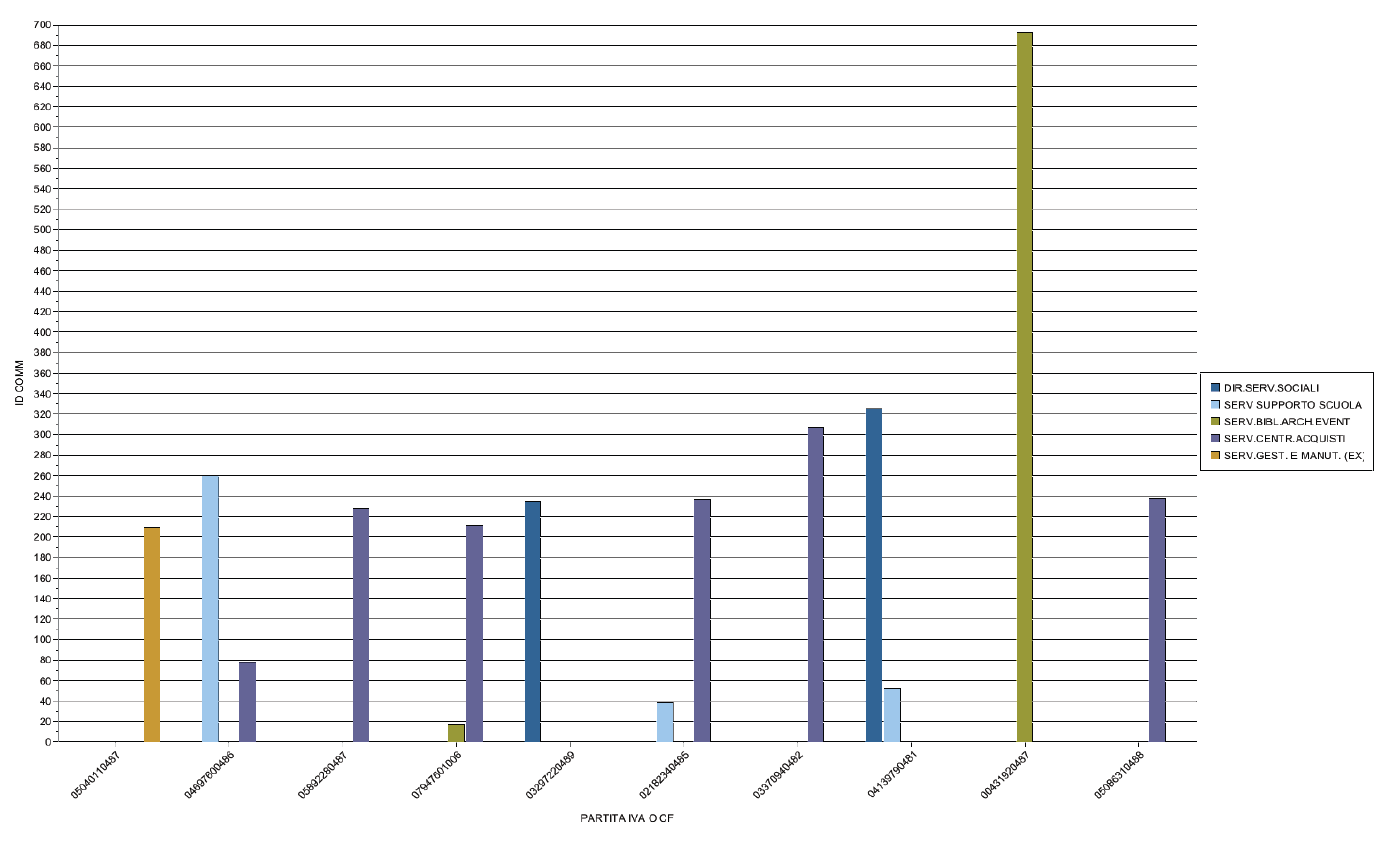
\includegraphics[scale=0.5]{top10_accoppiate.png}
			\caption{TOP 10 Accoppiate Direzione-Azienda, grafico.}
			\label{fig:top10_accoppiate}
		\end{figure}
		
		\begin{figure}[h!]
			\centering
				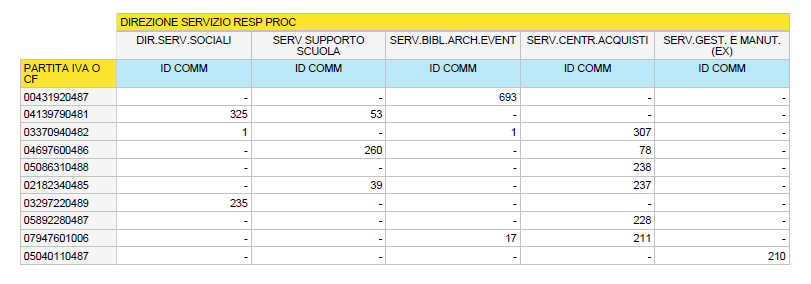
\includegraphics[scale=0.8]{top10_accoppiate_tab.png}
			\caption{TOP 10 Accoppiate Direzione-Azienda, tabella.}
			\label{fig:top10_accoppiate_tab}
		\end{figure}
		
		\begin{figure}[h!]
			\centering
				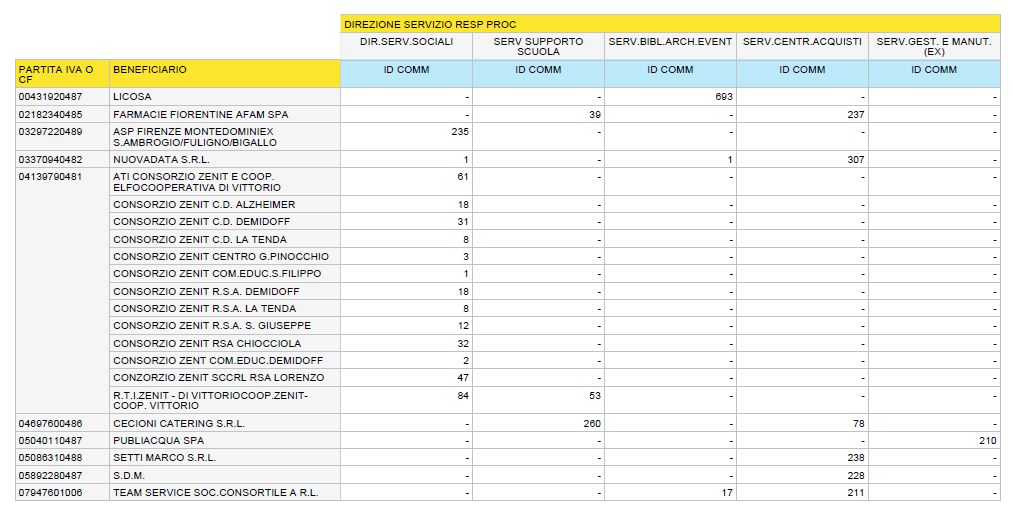
\includegraphics[scale=0.8]{top10_accoppiate_tab_dis.png}
			\caption{TOP 10 Accoppiate Direzione-Azienda, tabella disaggregata.}
			\label{fig:top10_accoppiate_tab_dis}
		\end{figure}
		
		Al primo posto, con ben 693 commissioni, troviamo la Direzione \textit{Servizi Biblioteche e Archivistica} e l'Azienda \textit{Licosa}. \textit{Licosa} è infatti un'Azienda fiorentina che si occupa di abbonamenti a riviste, fornitura e ricerca di libri e pubblicazioni.\\
		Al secondo posto troviamo invece la coppia \textit{Direzione Servizi Sociali} con il \textit{Consorzio Zenit} (che avevamo già citato in Sezione \ref{sec:pagamenti_aziende} tra le Aziende più pagate nel 2012/2013).
		
		\FloatBarrier
	
	\section{TOP 10 Anni di Pagamento per Aziende} \label{sec:anni_pagamento_aziende}
		
		Adesso ci proponiamo invece di individuare a quali Aziende, tra quelle presenti nei bilanci 2012/2013, sono stati assegnati i lavori più lunghi (e presumibilmente più impegnativi).
		
		\begin{figure}[h!]
			\centering
				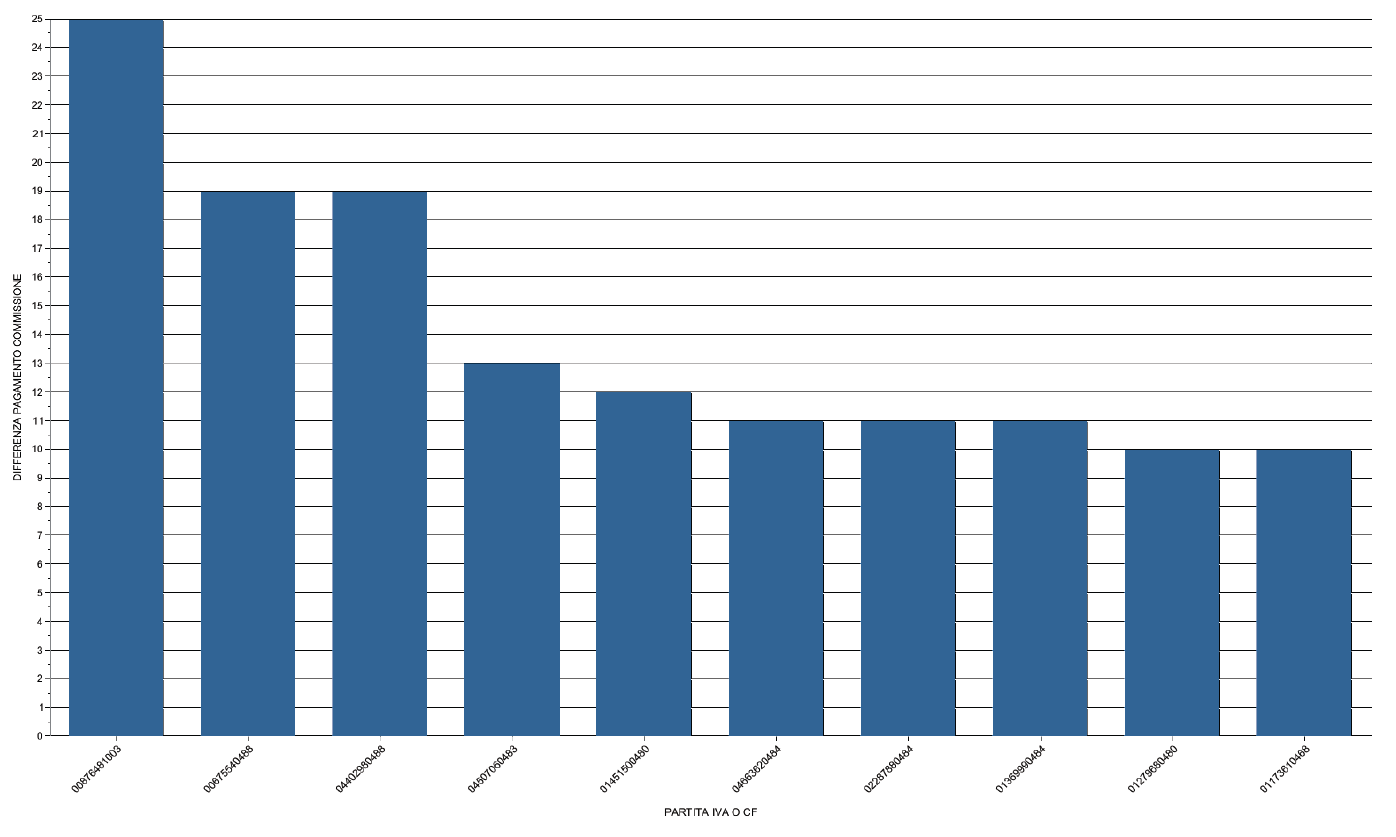
\includegraphics[scale=0.5]{top10_differenzepagamento_aziende.png}
			\caption{TOP 10 Anni di Pagamento per Aziende, grafico.}
			\label{fig:top10_differenzepagamento_aziende}
		\end{figure}
		
		\begin{figure}[h!]
			\centering
				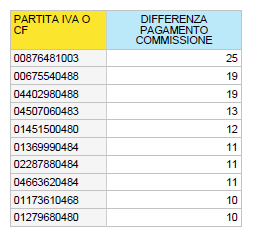
\includegraphics[scale=0.8]{top10_differenzepagamento_aziende_tab.png}
			\caption{TOP 10 Anni di Pagamento per Aziende, tabella.}
			\label{fig:top10_differenzepagamento_aziende_tab}
		\end{figure}
		
		\begin{figure}[h!]
			\centering
				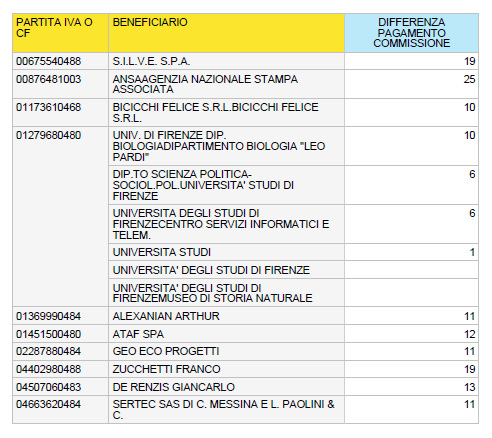
\includegraphics[scale=0.8]{top10_differenzepagamento_aziende_tab_dis.png}
			\caption{TOP 10 Anni di Pagamento per Aziende, tabella disaggregata.}
			\label{fig:top10_differenzepagamento_aziende_tab_dis}
		\end{figure}
		
		Al primo posto, con un lavoro durato ben 25 anni, troviamo l'\textit{ANSA} (\textit{Agenzia Nazionale Stampa Associata}), mentre al secondo e terzo posto, a pari merito con 19 anni, troviamo l'Azienda \textit{S.I.L.V.E. s.p.a.}, che si occupa di impianti di illuminazione elettrica, ed l'Azienda \textit{Zucchetti Franco}, i cui servizi ci sono ignoti. Le altre commissioni presenti in questa Top-10 vano invece dai 13 ai 10 anni di durata.
		
		\FloatBarrier
		
	\section{Analisi per tipo di Atto di Impegno} \label{sec:tipo_atto_impegno}
		
		Concludiamo questa serie di analisi con alcune osservazioni riguardanti il tipo di Atto di Impegno indicato per ogni commissione, ovvero sul campo \texttt{TIPO\_ATTO\_IMPEGNO} del nostro file \texttt{.csv}.\\
		Il tipo di Atto di Impegno è una sigla, di due o tre lettere, che indica con quale priorità è stato commissionato un certo mandato, ovvero l'importanza attribuita ad ogni commissione. A parte sigle poco utilizzate o deprecate, le due più importanti in questo senso sono \textit{DD} e \textit{CC}, che stanno, rispettivamente, per \textit{Decreto} (o \textit{Determina}) \textit{Dirigenziale} e per \textit{Consiglio Comunale}.\\
		Un \textit{Decreto Dirigenziale} indicherà quindi tutte quelle decisioni prese da un dirigente del settore (solitamente il dirigente della Direzione di Servizio che commissiona il lavoro), che non necessitano consiglio o approvazione da parte di altri settori; al contrario, un lavoro commissionato dal \textit{Consiglio Comunale} sarà sicuramente un lavoro molto più importante o impegnativo, in quanto richiede che tutto il Consiglio Comunale sia d'accordo sui dettagli e le modalità di quel particolare mandato.
		
		\subsection{\textit{Consigli Comunali} negli anni} \label{subsec:cc_negli_anni}
		
			Una prima, semplice analisi in questo senso può essere la determinazione di quanti mandati sono stati commissionati dal Consiglio Comunale negli anni, per capire in quale anno sono state prese più ``decisioni importanti''.\\
			Effettuiamo quindi un'analisi su due dimensioni: il tipo di Atto d'Impegno, che sarà fissato su \textit{CC}, e l'Anno di Commissione, che spazierà sull'intero dominio.\\
			
			\begin{figure}[h!]
				\centering
					\includegraphics[scale=0.5]{cc_2009-2013.png}
				\caption{\textit{Consigli Comunali} negli anni, grafico.}
				\label{fig:cc_2009-2013}
			\end{figure}
			
			\begin{figure}[h!]
				\centering
					\includegraphics[scale=0.8]{cc_2009-2013_tab.png}
				\caption{\textit{Consigli Comunali} negli anni, tabella.}
				\label{fig:cc_2009-2013_tab}
			\end{figure}
			
			Si osserva innanzitutto che prima del 2009 non è stato fatto (o più ragionevolmente, non è stato registrato) alcun \textit{Consiglio Comunale}, come anche nel 2013. Quindi per quanto riguarda gli anni che vanno dal 2009 al 2012, si vede che la differenza tra i vari anni è minima, raggiungendo un picco nel 2011, con 33 \textit{Consigli Comunali}.
			
			\FloatBarrier
			
		\subsection{Confronto: CC-DD nel 2009-2013} \label{subsec:cc-dd_2009-2013}
		
			Volendo entrare adesso più nel dettaglio rispetto all'analisi precedente, possiamo includere anche il numero, per ogni anno, di lavori approvati per \textit{Decreto Dirigenziale}, mettendo in relazione quanti lavori sono stati commissionati per \textit{Consiglio Comunale} e quanti per \textit{Decreto Dirigenziale}.\\
			
			\begin{figure}[h!]
				\centering
					\includegraphics[scale=0.5]{cc-dd_2009-2013_a.png}
				\caption{\textit{Consigli Comunali} e \textit{Decreti Dirigenziali} negli anni, grafico a linee.}
				\label{fig:cc-dd_2009-2013_a}
			\end{figure}
			
			\begin{figure}[h!]
				\centering
					\includegraphics[scale=0.5]{cc-dd_2009-2013_b.png}
				\caption{\textit{Consigli Comunali} e \textit{Decreti Dirigenziali} negli anni, grafici a torta.}
				\label{fig:cc-dd_2009-2013_b}
			\end{figure}
			
			\begin{figure}[h!]
				\centering
					\includegraphics[scale=0.8]{cc-dd_2009-2013_tab.png}
				\caption{\textit{Consigli Comunali} e \textit{Decreti Dirigenziali} negli anni, tabella.}
				\label{fig:cc-dd_2009-2013_tab}
			\end{figure}
			
			Come ci si poteva aspettare, i \textit{Decreti Dirigenziali}, associati a lavori più semplici o meno importanti, sono molti di più rispetto ai \textit{Consigli Comunali}, come possiamo vedere sia dai grafici che dalla tabella. Inoltre, se osserviamo i grafici a torta in Figura \ref{fig:cc-dd_2009-2013_b}, si nota anche che in percentuale i \textit{Consigli Comunali} sono andati a diminuire negli anni rispetto ai \textit{Decreti Dirigenziali}. Escludendo motivi tecnici del settore (sui quali non possiamo fare speculazioni di alcun tipo), una possibile spiegazione potrebbe essere che, essendo i \textit{Consigli Comunali} molto più importanti di un qualsiasi \textit{Decreto Dirigenziale}, questi sono stati tracciati e registrati in modo più accurato e preciso rispetto ai \textit{Decreti Dirigenziali}, che molto probabilmente venivano persi tra le scartoffie e la burocrazia del Comune, almeno fino al Decreto Sviluppo 2012.
			
			\FloatBarrier
	\chapter{Conclusioni} \label{chap:conclusioni}

    Concludiamo questa tesi con alcune riflessioni sul lavoro svolto.
    
    Il Progetto KT per Indico è stato sicuramente molto utile per il progetto Indico in quanto ha aggiunto molte funzionalità che prima mancavano e che certamente lo renderanno più visibile al mondo esterno, anziché esclusivamente all'interno del \ac{CERN} e dell'ambiente della fisica delle particelle.
    
    Grazie al progetto di Cloud Deployment è adesso possibile, tramite un semplice script, installare Indico su una macchina virtuale o installarlo, da remoto, su un server cloud. Inoltre, grazie allo script di gestione, è anche resa più facile all'utente la gestione dell'istanza di Indico installata su macchina virtuale, fornendo una maggior destrezza di utilizzo.
    
    Lo script fabric per le distribuzioni di Indico ha invece reso certamente la vita più facile al team di sviluppo di Indico al \ac{CERN} che adesso potranno, tramite l'invocazione di un solo comando, creare nuove distribuzioni di Indico e caricarle su un server o su GitHub in maniera completamente automatica.
    
    Il progetto di Instance Tracking si è rivelato essere il più importante tra tutti in quanto ha portato allo sviluppo di un'applicazione completamente nuova e indipendente da Indico: Cephalopod. Grazie a Cephalopod sarà adesso possibile tracciare e creare statistiche sulle istanze di Indico installate in tutto il mondo. Non solo, Cephalopod riveste un ruolo ancora più importante in quanto è utilizzabile non soltanto da Indico, ma anche da altre applicazioni web che intendono tracciare le proprie istanze, sia al \ac{CERN} che altrove.
    
    L'ultima fase del progetto, anche se non molto rilevante dal punto di vista implementativo, è invece stata molto utile in quanto ha stabilito le basi di sviluppo sul quale il team di Indico andrà a creare, in futuro, un nuovo tool per la creazione e la personalizzazione di conferenze che sarà basato sul sistema ibrido blocco-widget ed implementerà un'intuitiva interfaccia drag-and-drop.
    
    Concludendo, l'esperienza al \ac{CERN} è stata un'esperienza altamente formativa, sia dal punto di vista professionale, permettendo di studiare ed utilizzare molti strumenti e linguaggi nuovi, che umano. Infatti, oltre all'aspetto lavorativo, i 14 mesi passati a Ginevra hanno portato ad un arricchimento e ad una crescita sotto molti punti di vista, che trascendono il semplice ambito professionale.

	
	\nocite{*}
	\bibliographystyle{plainnat}
	\bibliography{bibliografia}

\end{document}